
\labday{Mardi, 24 mai 2016}
\label{day:24-05-2016}

Aujourd'hui, je vais rassembler l'intégralité des résultats dans ce cahier.
Tous les toys, toutes les transformations linéaires et même un petit bonus avec
la grille tordue !

L'objectif étant de faire une compilation des expérimentations faites jusqu'à présent
avec le correcteur linéaire.

\experiment{Rappels}

L'objectif de ces expériences est d'arriver à associer entre-elles des données
provenant de distributions très similaires.

\begin{itemize}
	\item $\mathcal{X_S}$: données \textbf{Sources} \textbf{Originales}, \textbf{Non biaisées}, \textbf{Réalité}.
	\item $\mathcal{X_T}$: données \textbf{Cible}, \textbf{Transformées}, \textbf{biaisées}, \textbf{Simulations}.
	\item $\phi$: la \textbf{transformation}, le \textbf{biais}
	\item $\psi$: le \textbf{correcteur}, un réseau de neurone
\end{itemize}
On cherche : $\phi \circ \psi = identity$.

\textbf{L'alignement} est l'information qu'un point $x_i$ des données \emph{Sources} correspond 
à $x_i^\prime$ des données \emph{Cibles}. Cette information n'étant pas nécessairement 
disponnible dans les cas réels, on étudit les méthodes avec et sans cette information. 


Dans la suite je vais rassembler les résultats d'expérimentations par:
\begin{itemize}
	\item Jeu de donnée
	\begin{itemize}
		\item Méthode d'alignement
		\begin{itemize}
			\item Transformation
		\end{itemize}
	\end{itemize}
\end{itemize}
%%%%%%%%%%%%%%%%%%%%%%%%%%%%%%%%%%%%%%%%%%%%%%%%%%%%%%%%%%%%%%%%%%%%%%%%%%%%%%
%%%%%% CLOUDS
%%%%%%%%%%%%%%%%%%%%%%%%%%%%%%%%%%%%%%%%%%%%%%%%%%%%%%%%%%%%%%%%%%%%%%%%%%%%%%

\experiment{Clouds}

\emph{Clouds} est un jouet composé de $n$ classes (nuages de point gaussiens) se partageant 
l'espace sur le cercle unité.

Toutes ces expériences ont été réalisées avec un learning rate de $0.1$ + un moment de $0.9$.


\subexperiment{Alignement connu}

Le cas où l'alignement est connu permet de vérifier que la transformation est facile ou non 
à inverser, les autres méthode ayant peu de chance de faire mieux.

{\Large \textbf{Rotation :}}  On applique une rotation de 35 degrés par rapport à l'origine $(0,0)$.

\begin{figure}[H] % images
\centering
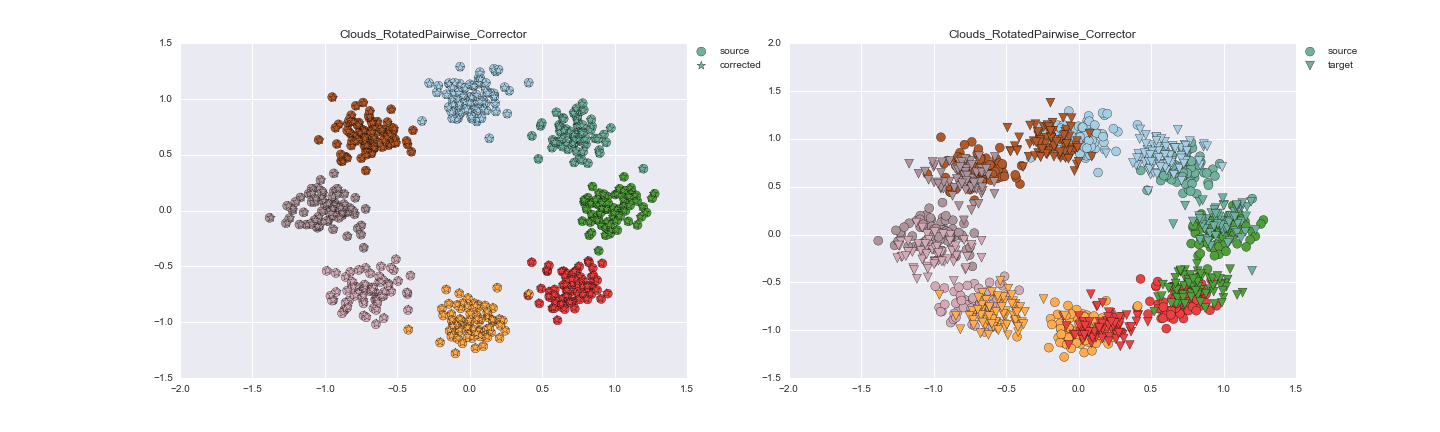
\includegraphics[width=\linewidth]{fig/24-05-2016/clouds/Clouds_RotatedPairwise_Corrector-DATA.png}
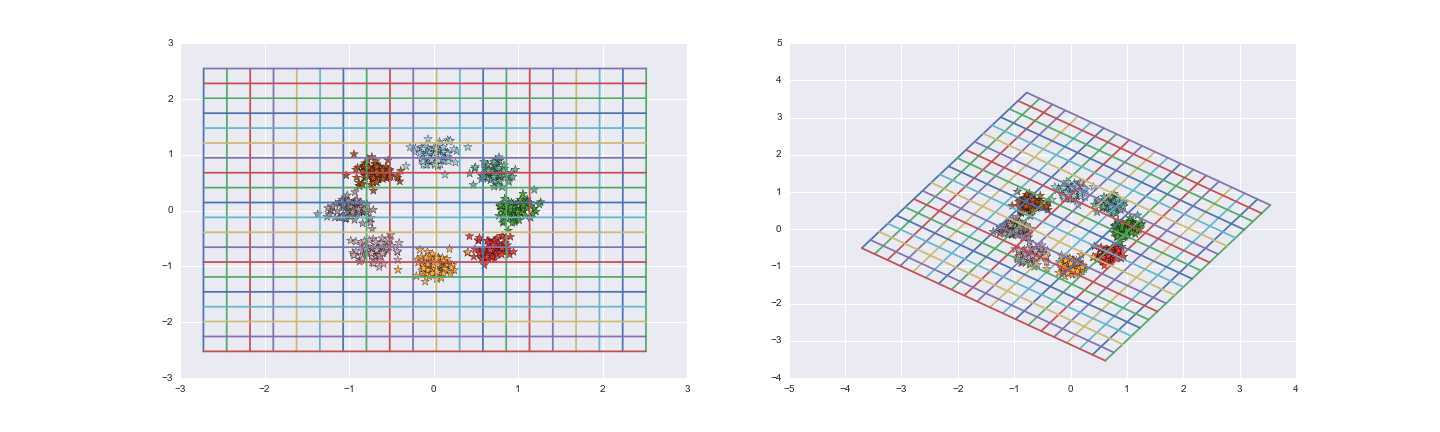
\includegraphics[width=\linewidth]{fig/24-05-2016/clouds/Clouds_RotatedPairwise_Corrector-GridCheck.png}
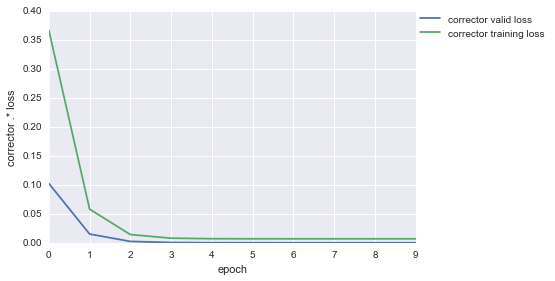
\includegraphics[width=0.45\linewidth]{fig/24-05-2016/clouds/Clouds_RotatedPairwise_Corrector-Learning_curve.png}
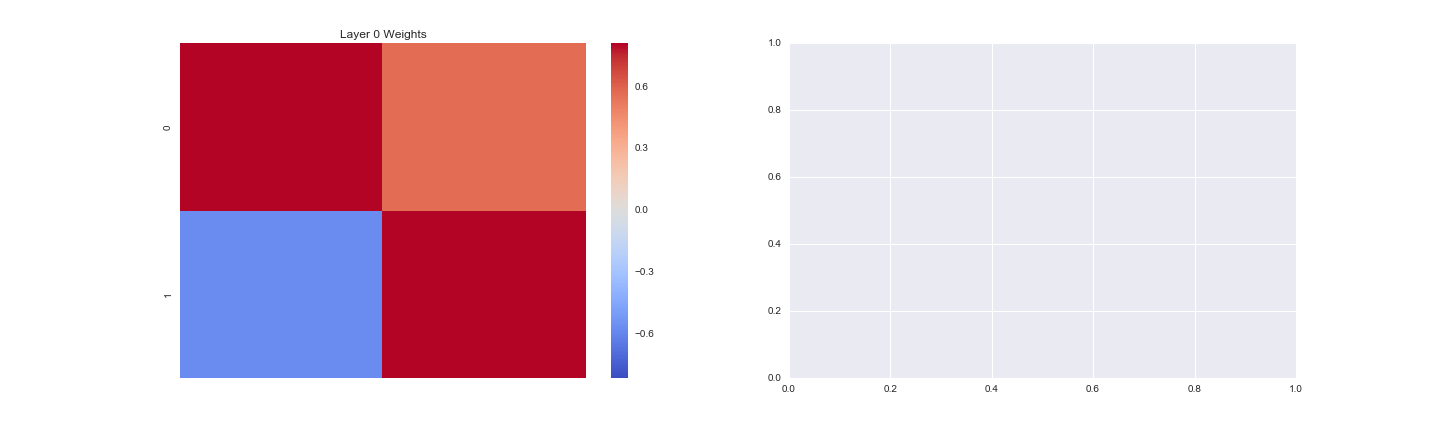
\includegraphics[width=\linewidth]{fig/24-05-2016/clouds/Clouds_RotatedPairwise_Corrector-W.png}
\caption{Correction de Clouds après une rotation de 35 degrés par rapport à l'origine avec alignement connu}
\label{fig:recap-clouds-rot-pairwise}
\end{figure}

{\Large \textbf{Random matrix :}}

\begin{figure}[H] % images
\centering
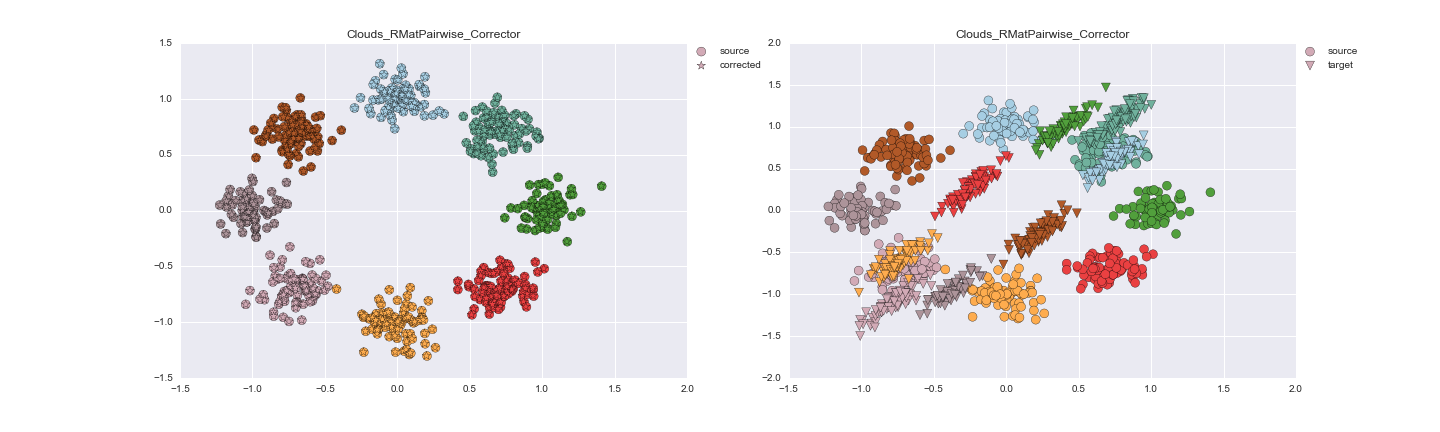
\includegraphics[width=\linewidth]{fig/24-05-2016/clouds/Clouds_RMatPairwise_Corrector-DATA.png}
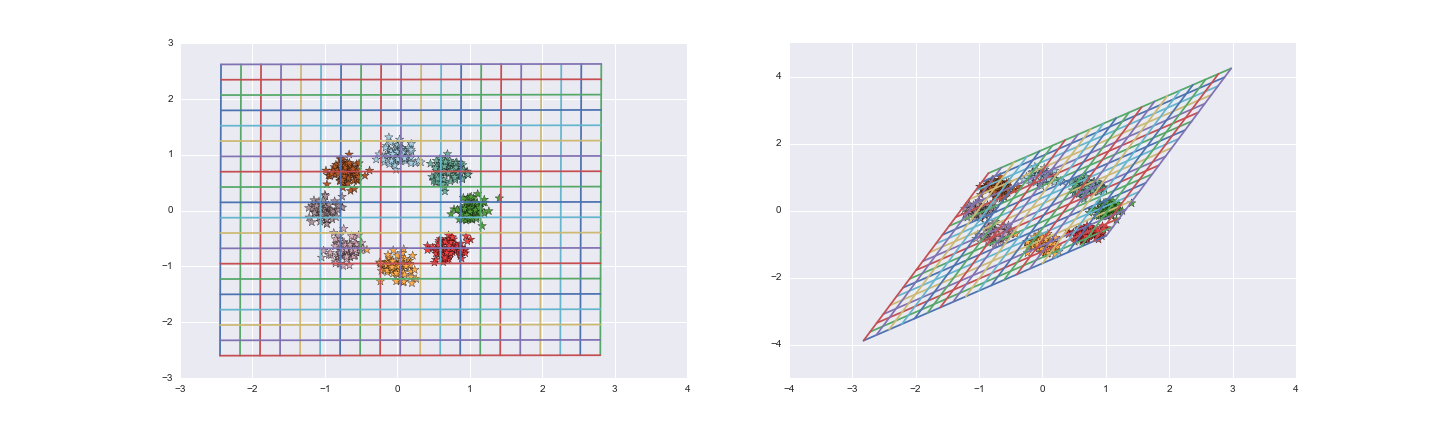
\includegraphics[width=\linewidth]{fig/24-05-2016/clouds/Clouds_RMatPairwise_Corrector-GridCheck.png}
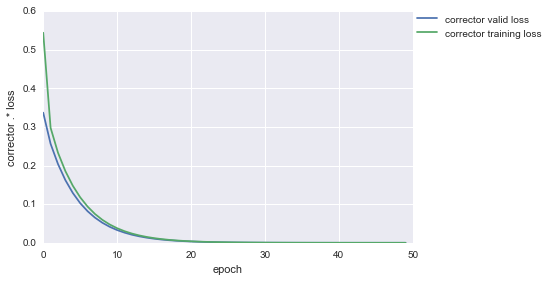
\includegraphics[width=0.45\linewidth]{fig/24-05-2016/clouds/Clouds_RMatPairwise_Corrector-Learning_curve.png}
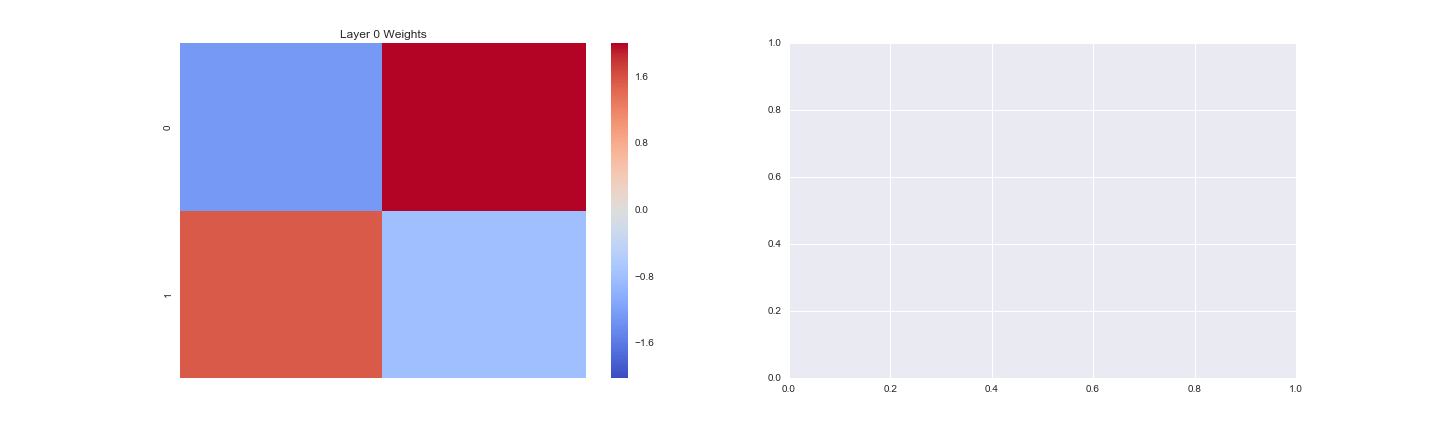
\includegraphics[width=\linewidth]{fig/24-05-2016/clouds/Clouds_RMatPairwise_Corrector-W.png}
\caption{Correction de Clouds après multiplication par une matrice générée aléatoirement}
\label{fig:recap-clouds-RMat-pairwise}
\end{figure}


{\Large \textbf{Grille tordue :}}

\begin{figure}[H] % images
\centering
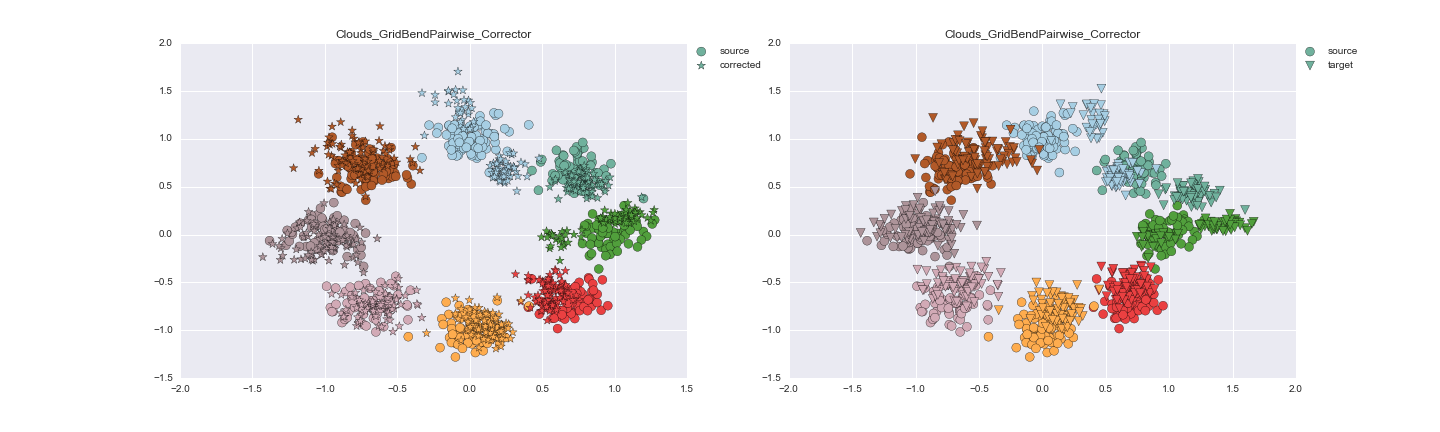
\includegraphics[width=\linewidth]{fig/24-05-2016/clouds/Clouds_GridBendPairwise_Corrector-DATA.png}
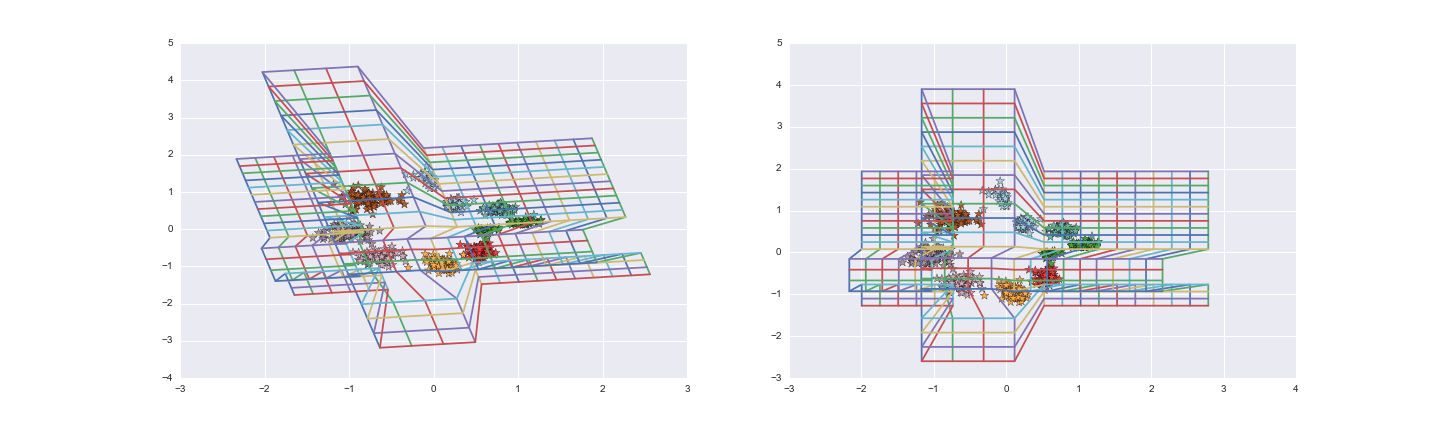
\includegraphics[width=\linewidth]{fig/24-05-2016/clouds/Clouds_GridBendPairwise_Corrector-GridCheck.png}
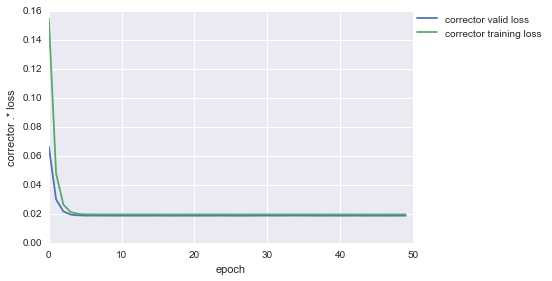
\includegraphics[width=0.45\linewidth]{fig/24-05-2016/clouds/Clouds_GridBendPairwise_Corrector-Learning_curve.png}
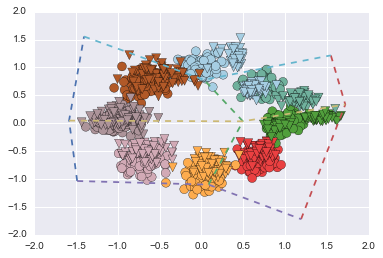
\includegraphics[width=0.45\linewidth]{fig/24-05-2016/clouds/cloud_grid.png}
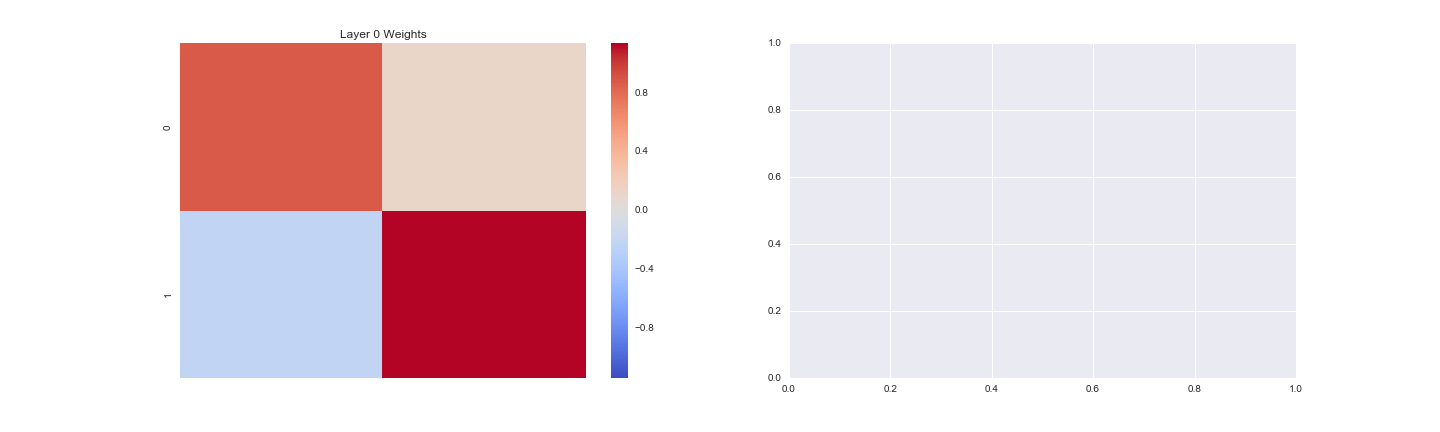
\includegraphics[width=\linewidth]{fig/24-05-2016/clouds/Clouds_GridBendPairwise_Corrector-W.png}
\caption{Correction de Clouds après application d'une transformation linéaire locale}
\label{fig:recap-clouds-GridBend-pairwise}
\end{figure}

\subexperiment{Alignement appris : alignement aléatoire au sein des classes}

{\Large \textbf{Rotation :}} On applique une rotation de 35 degrés par rapport à l'origine $(0,0)$.

\begin{figure}[H] % images
\centering
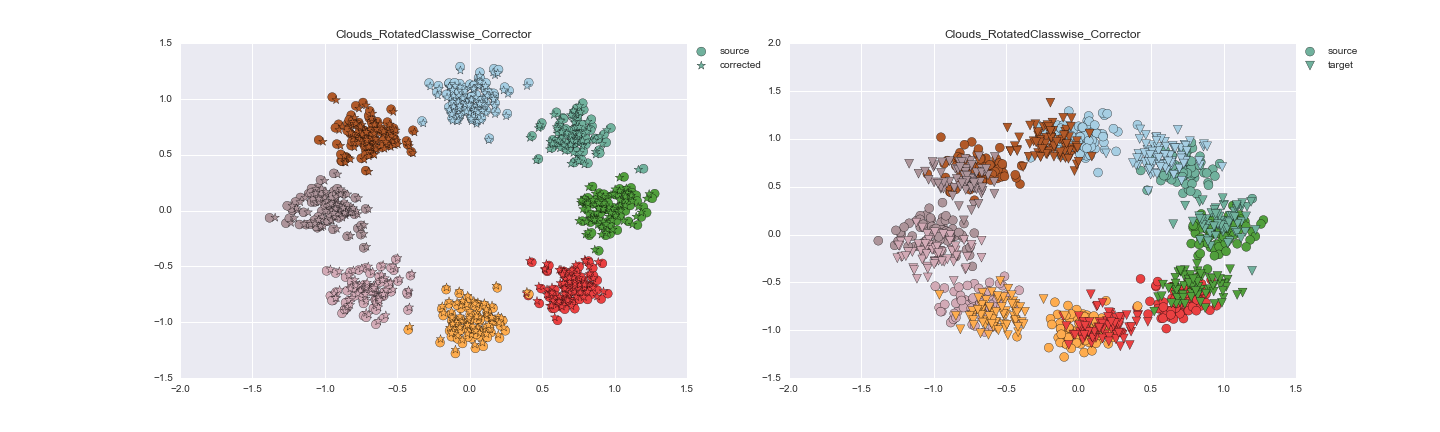
\includegraphics[width=\linewidth]{fig/24-05-2016/clouds/Clouds_RotatedClasswise_Corrector-DATA.png}
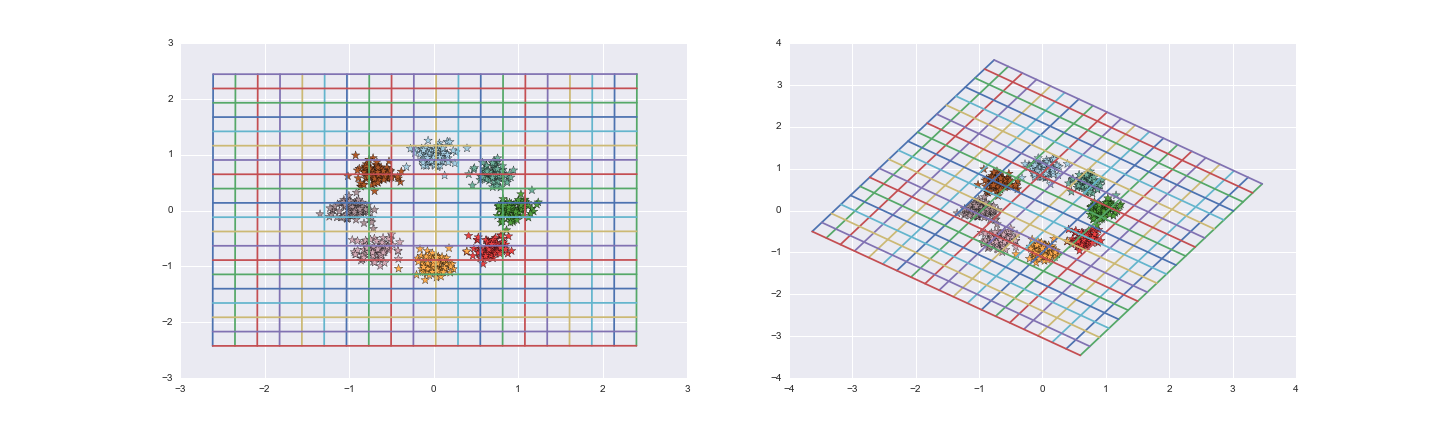
\includegraphics[width=\linewidth]{fig/24-05-2016/clouds/Clouds_RotatedClasswise_Corrector-GridCheck.png}
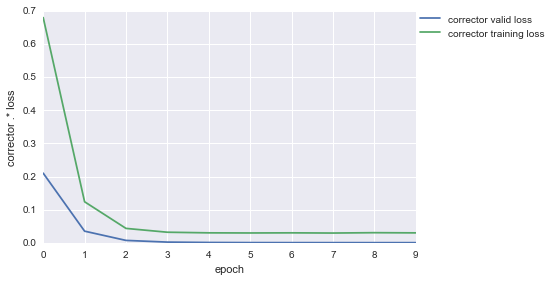
\includegraphics[width=0.45\linewidth]{fig/24-05-2016/clouds/Clouds_RotatedClasswise_Corrector-Learning_curve.png}
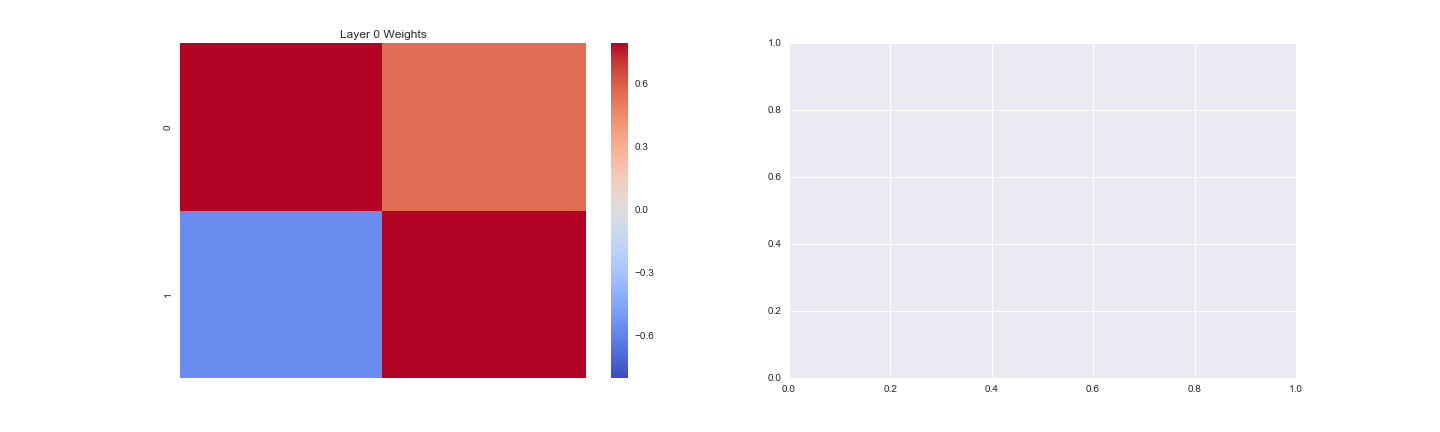
\includegraphics[width=\linewidth]{fig/24-05-2016/clouds/Clouds_RotatedClasswise_Corrector-W.png}
\caption{Correction de Clouds après une rotation de 35 degrés par rapport à l'origine avec les plus proches voisins entre les clusters}
\label{fig:recap-clouds-rot-classwise}
\end{figure}

{\Large \textbf{Random matrix :}}

\begin{figure}[H] % images
\centering
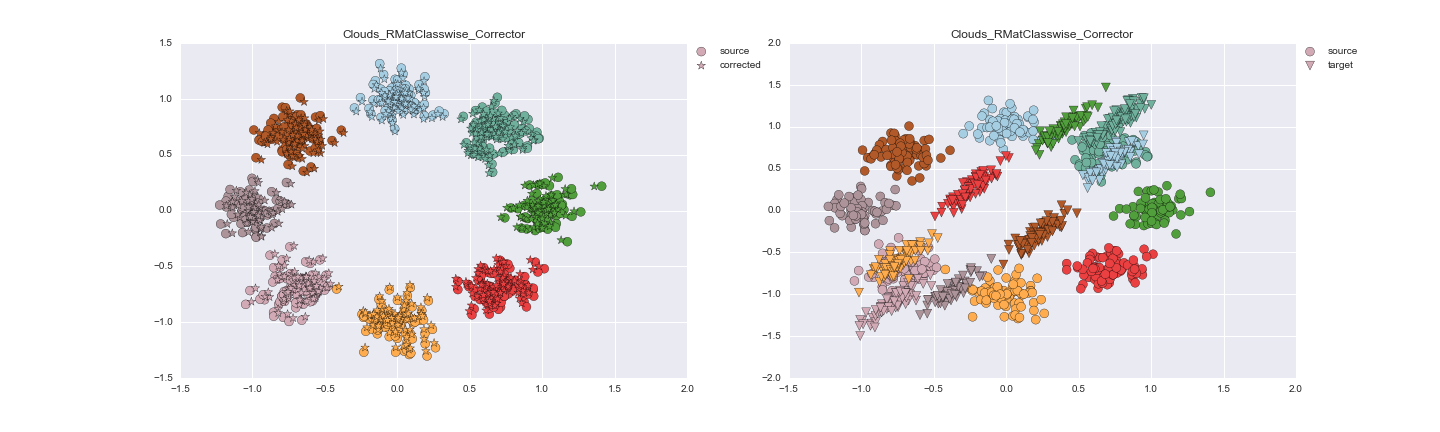
\includegraphics[width=\linewidth]{fig/24-05-2016/clouds/Clouds_RMatClasswise_Corrector-DATA.png}
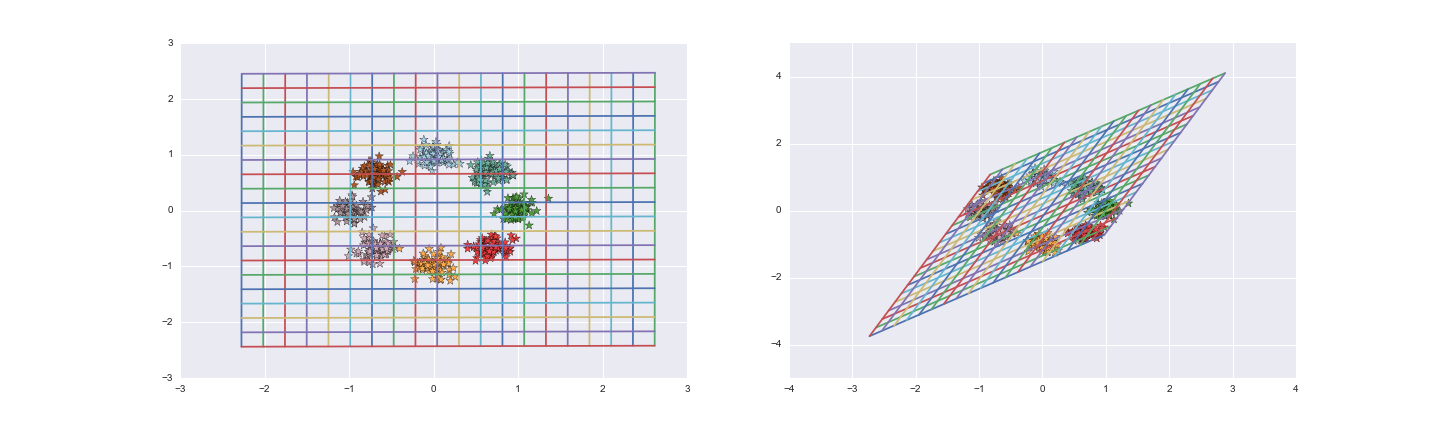
\includegraphics[width=\linewidth]{fig/24-05-2016/clouds/Clouds_RMatClasswise_Corrector-GridCheck.png}
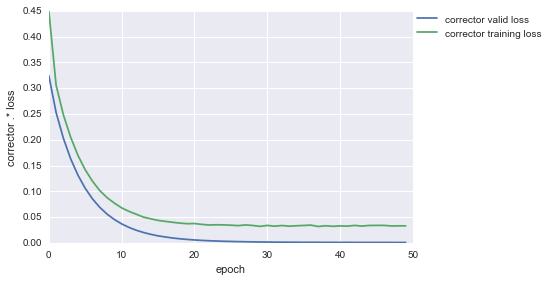
\includegraphics[width=0.45\linewidth]{fig/24-05-2016/clouds/Clouds_RMatClasswise_Corrector-Learning_curve.png}
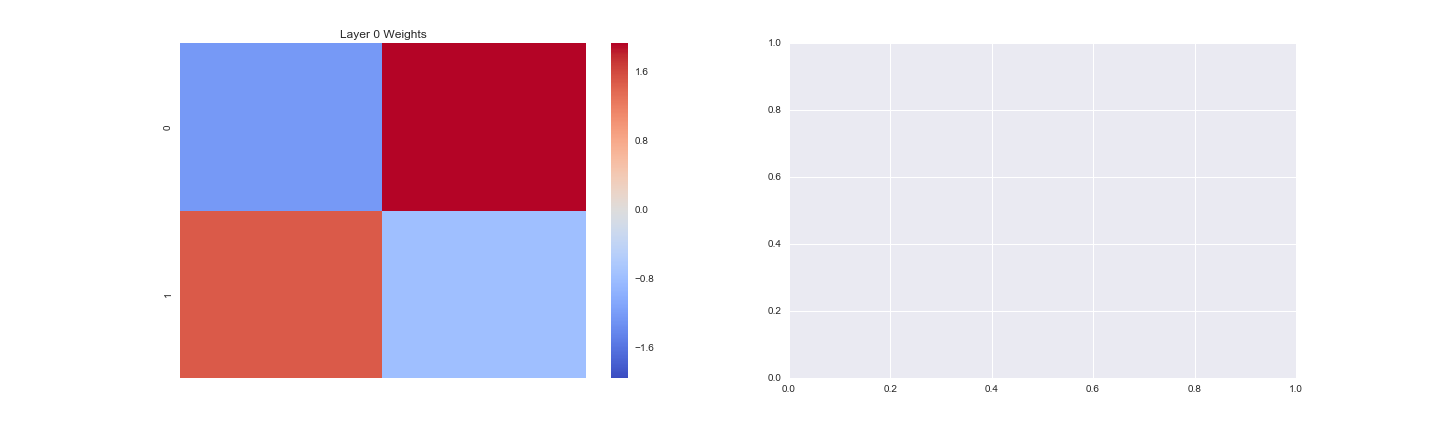
\includegraphics[width=\linewidth]{fig/24-05-2016/clouds/Clouds_RMatClasswise_Corrector-W.png}
\caption{Correction de Clouds après multiplication par une matrice générée aléatoirement}
\label{fig:recap-clouds-RMat-classwise}
\end{figure}

{\Large \textbf{Grille tordue :}}

\begin{figure}[H] % images
\centering
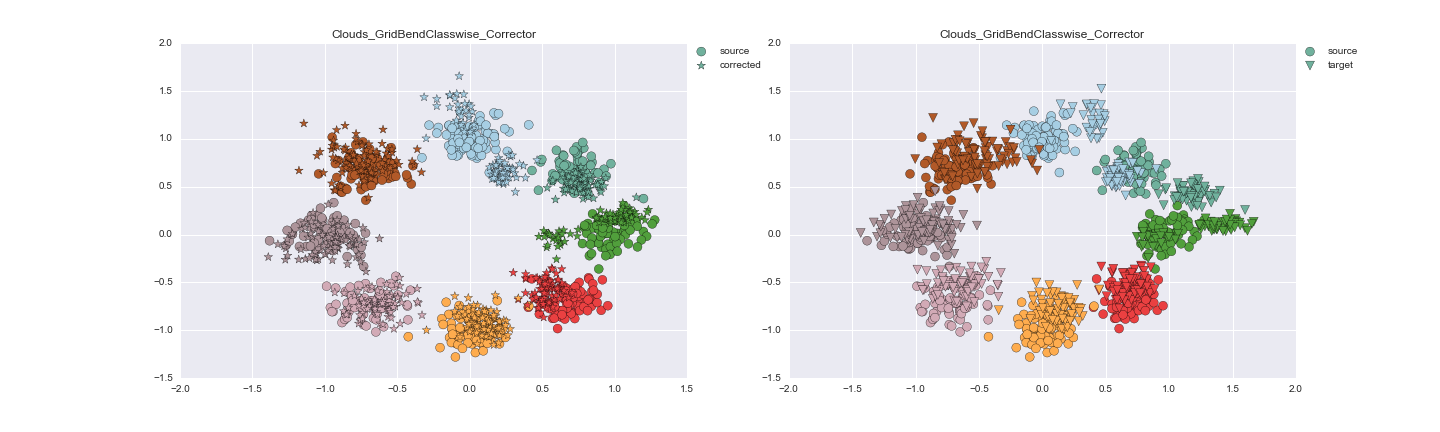
\includegraphics[width=\linewidth]{fig/24-05-2016/clouds/Clouds_GridBendClasswise_Corrector-DATA.png}
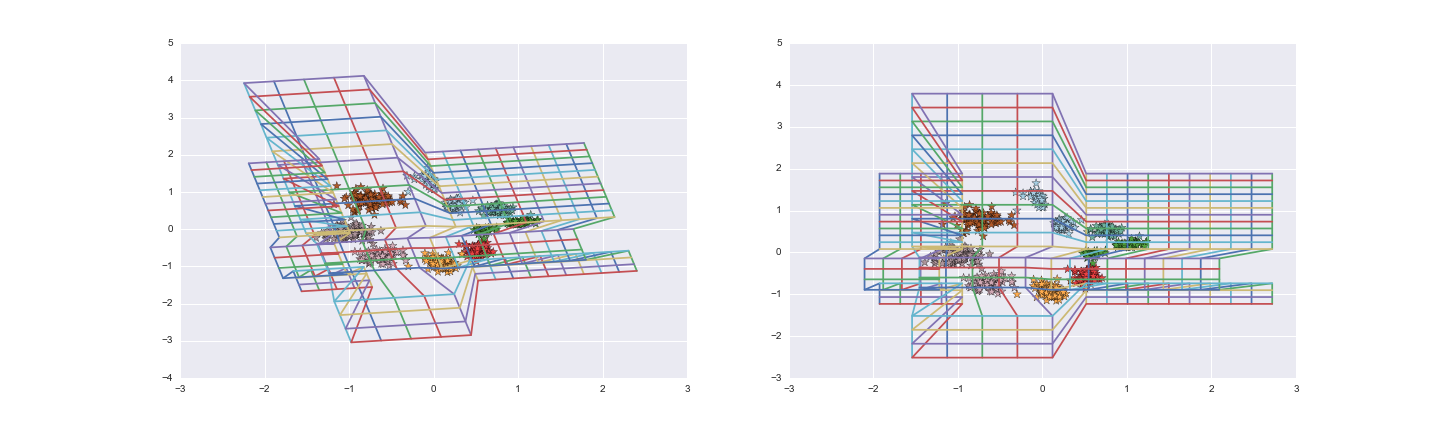
\includegraphics[width=\linewidth]{fig/24-05-2016/clouds/Clouds_GridBendClasswise_Corrector-GridCheck.png}
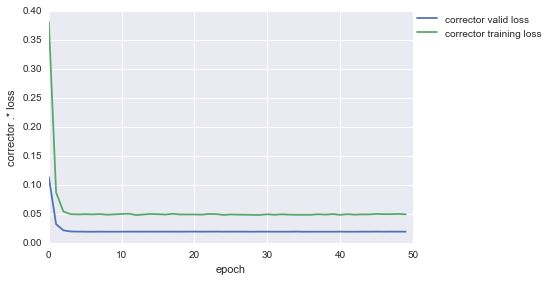
\includegraphics[width=0.45\linewidth]{fig/24-05-2016/clouds/Clouds_GridBendClasswise_Corrector-Learning_curve.png}
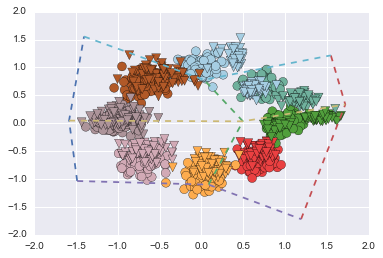
\includegraphics[width=0.45\linewidth]{fig/24-05-2016/clouds/cloud_grid.png}
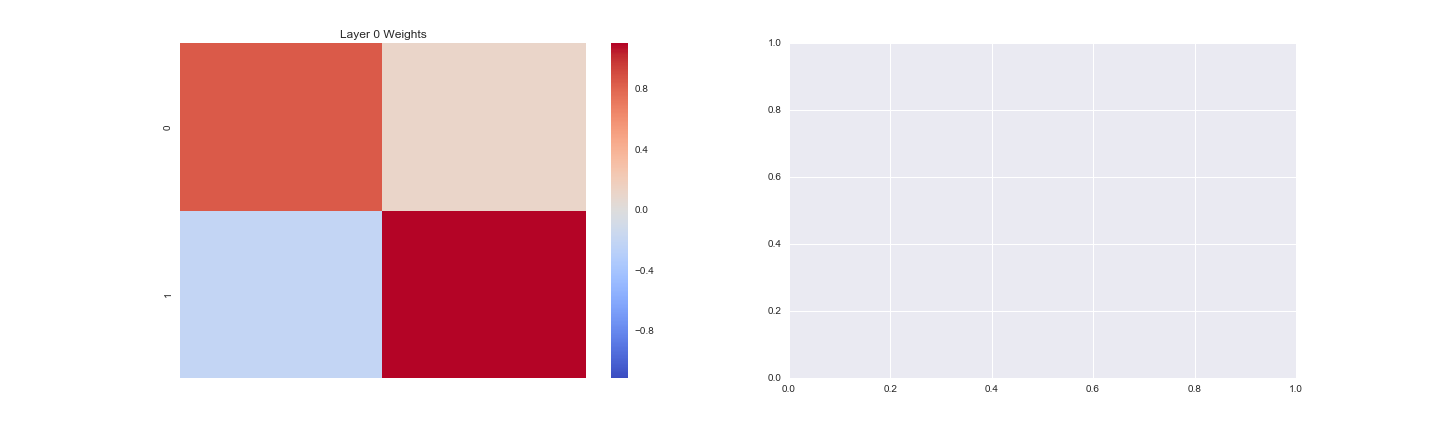
\includegraphics[width=\linewidth]{fig/24-05-2016/clouds/Clouds_GridBendClasswise_Corrector-W.png}
\caption{Correction de Clouds après application d'une transformation linéaire locale}
\label{fig:recap-clouds-GridBend-classwise}
\end{figure}


\subexperiment{Alignement appris : alignement au plus proche voisin au sein des classes}

{\Large \textbf{Rotation :}} On applique une rotation de 35 degrés par rapport à l'origine $(0,0)$.

\begin{figure}[H] % images
\centering
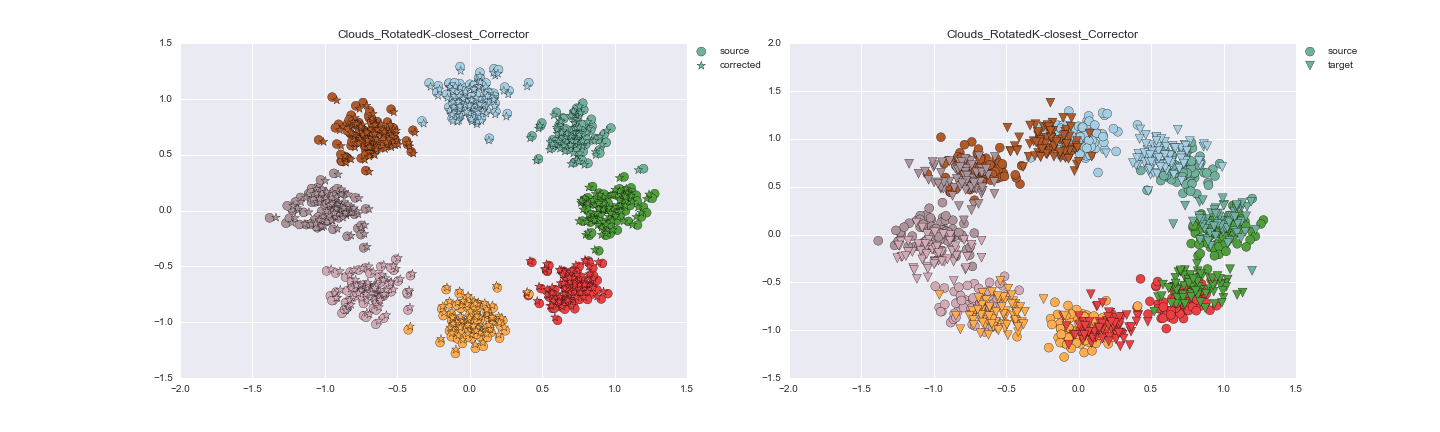
\includegraphics[width=\linewidth]{fig/24-05-2016/clouds/Clouds_RotatedK-closest_Corrector-DATA.png}
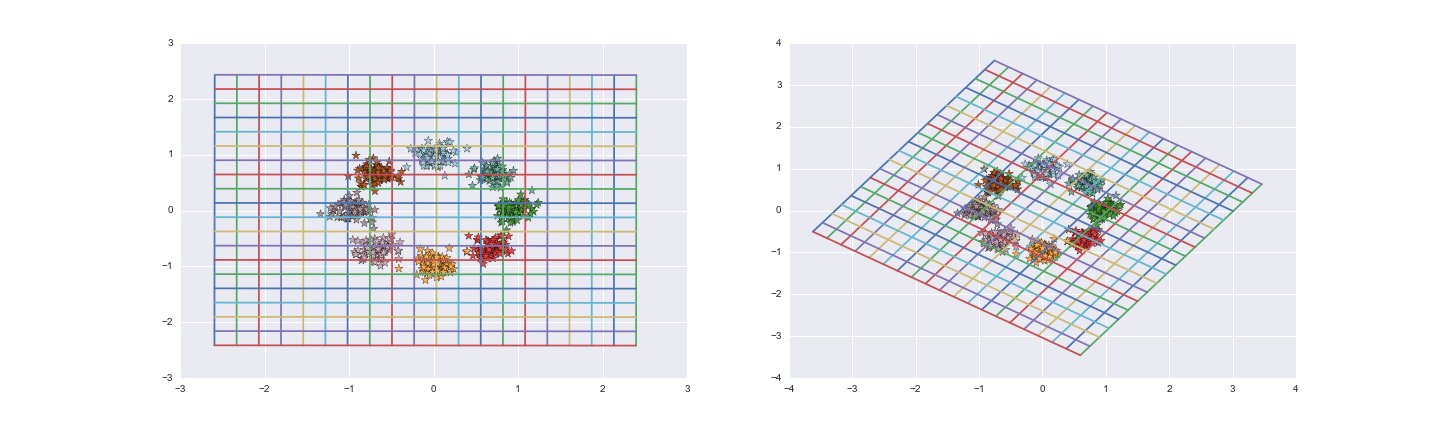
\includegraphics[width=\linewidth]{fig/24-05-2016/clouds/Clouds_RotatedK-closest_Corrector-GridCheck.png}
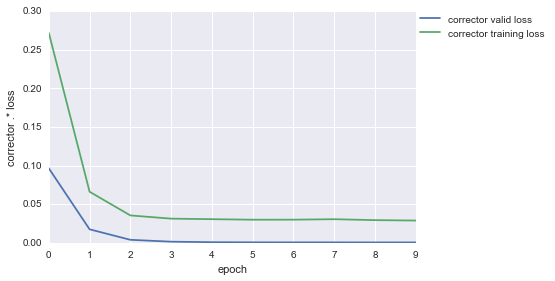
\includegraphics[width=0.45\linewidth]{fig/24-05-2016/clouds/Clouds_RotatedK-closest_Corrector-Learning_curve.png}
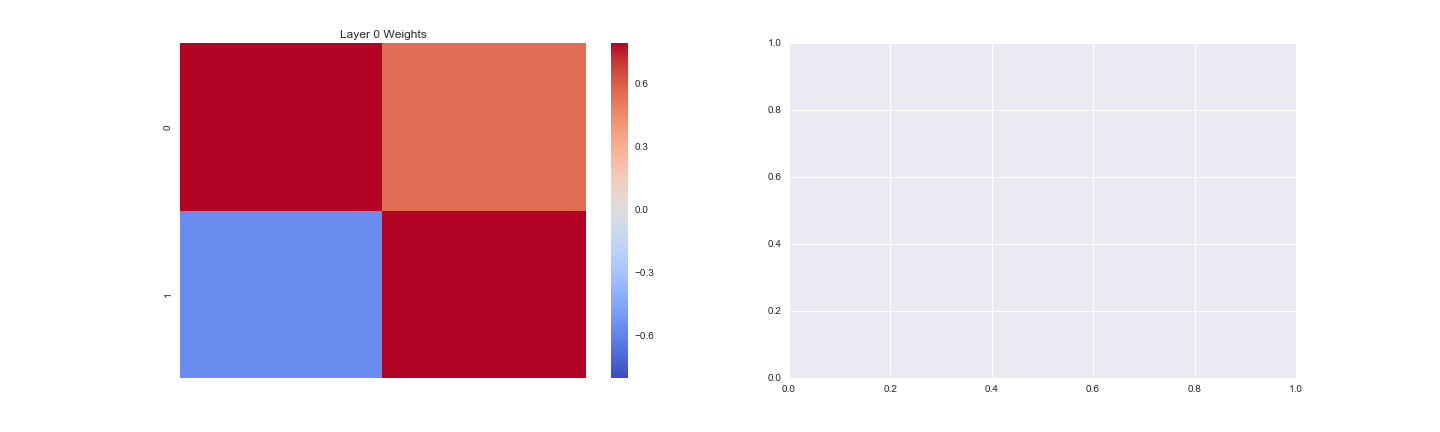
\includegraphics[width=\linewidth]{fig/24-05-2016/clouds/Clouds_RotatedK-closest_Corrector-W.png}
\caption{Correction de Clouds après une rotation de 35 degrés par rapport à l'origine avec les plus proches voisins entre les clusters}
\label{fig:recap-clouds-rot-exhaustive}
\end{figure}

{\Large \textbf{Random matrix :}}

\begin{figure}[H] % images
\centering
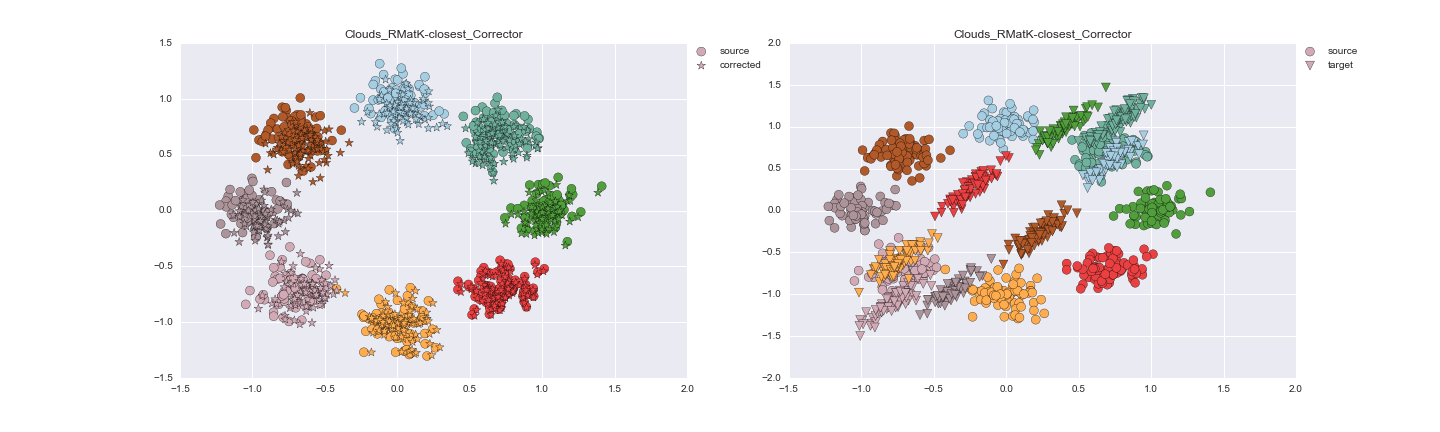
\includegraphics[width=\linewidth]{fig/24-05-2016/clouds/Clouds_RMatK-closest_Corrector-DATA.png}
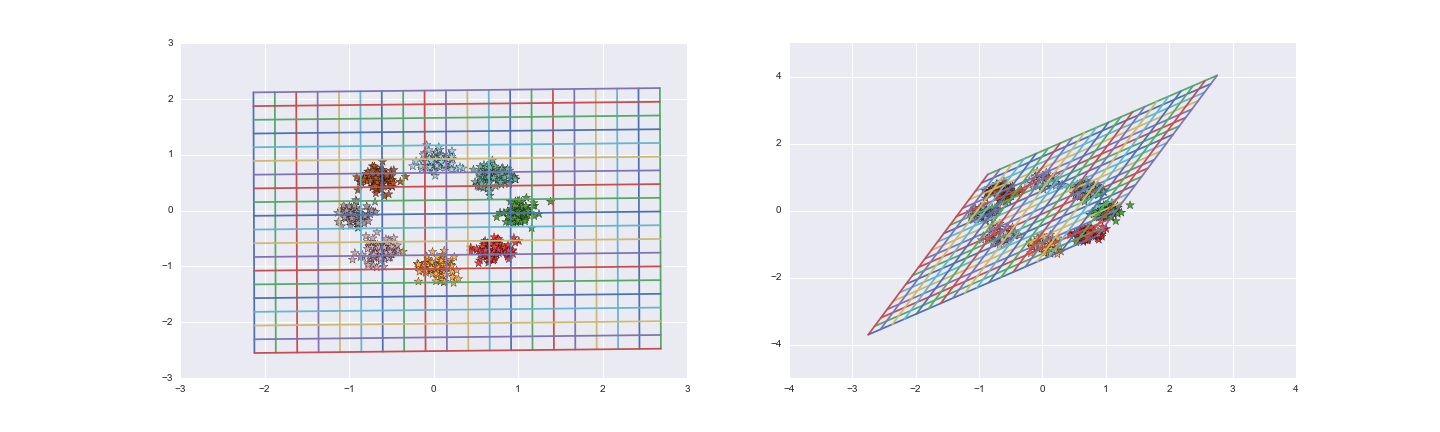
\includegraphics[width=\linewidth]{fig/24-05-2016/clouds/Clouds_RMatK-closest_Corrector-GridCheck.png}
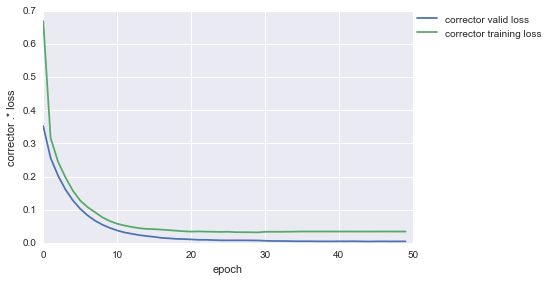
\includegraphics[width=0.45\linewidth]{fig/24-05-2016/clouds/Clouds_RMatK-closest_Corrector-Learning_curve.png}
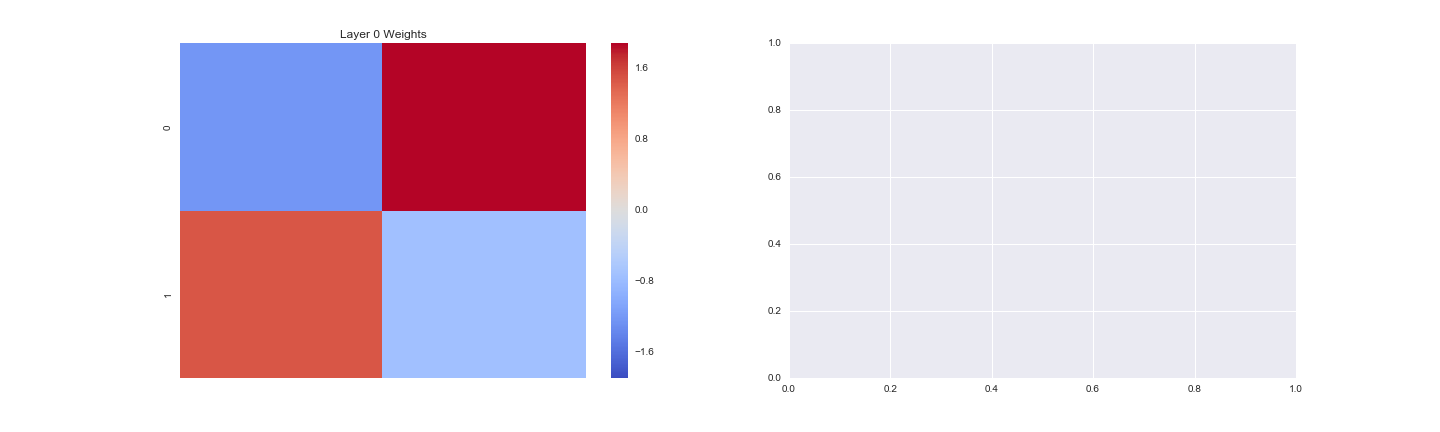
\includegraphics[width=\linewidth]{fig/24-05-2016/clouds/Clouds_RMatK-closest_Corrector-W.png}
\caption{Correction de Clouds après multiplication par une matrice générée aléatoirement}
\label{fig:recap-clouds-RMat-exhaustive}
\end{figure}

{\Large \textbf{Grille tordue :}}

\begin{figure}[H] % images
\centering
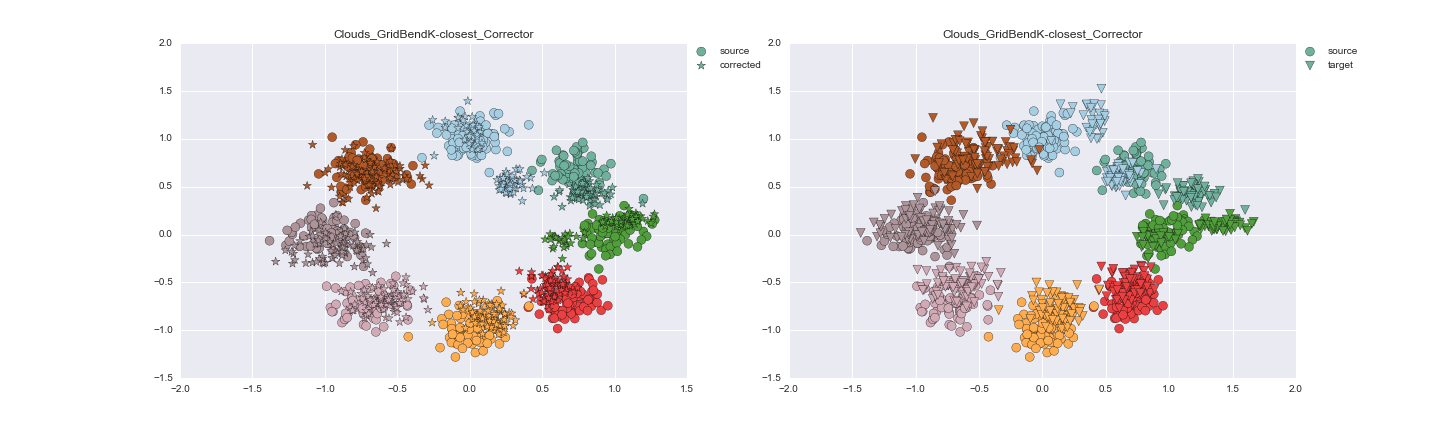
\includegraphics[width=\linewidth]{fig/24-05-2016/clouds/Clouds_GridBendK-closest_Corrector-DATA.png}
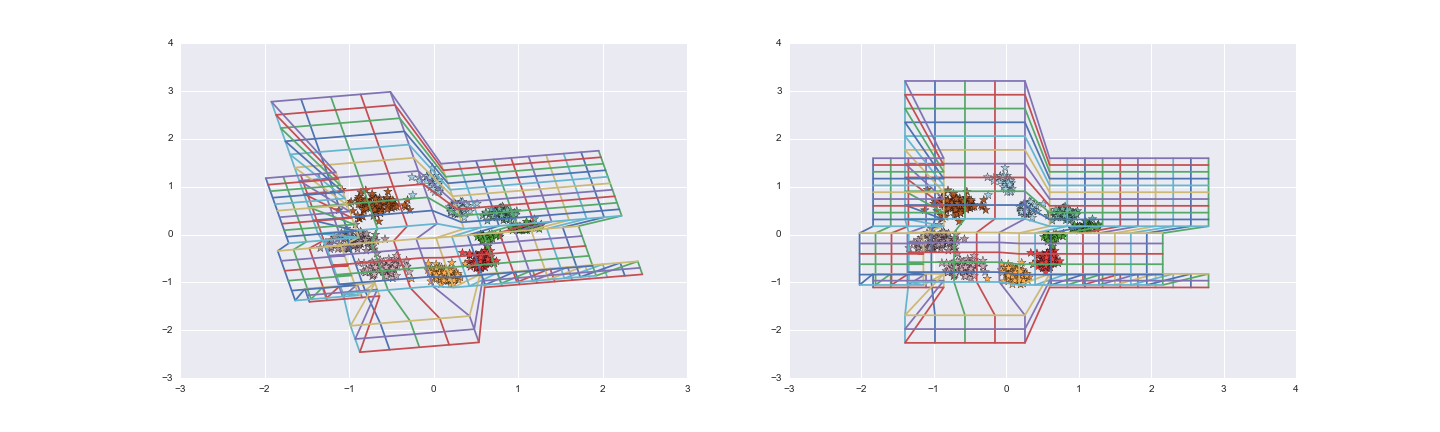
\includegraphics[width=\linewidth]{fig/24-05-2016/clouds/Clouds_GridBendK-closest_Corrector-GridCheck.png}
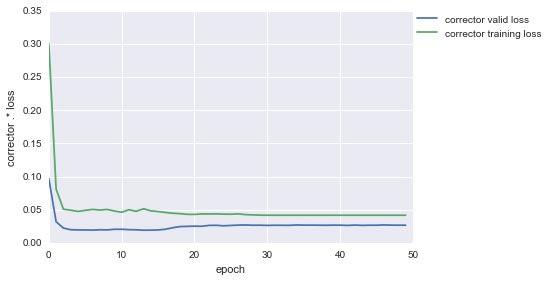
\includegraphics[width=0.45\linewidth]{fig/24-05-2016/clouds/Clouds_GridBendK-closest_Corrector-Learning_curve.png}
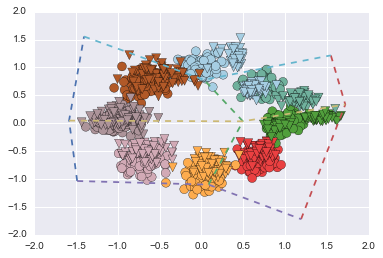
\includegraphics[width=0.45\linewidth]{fig/24-05-2016/clouds/cloud_grid.png}
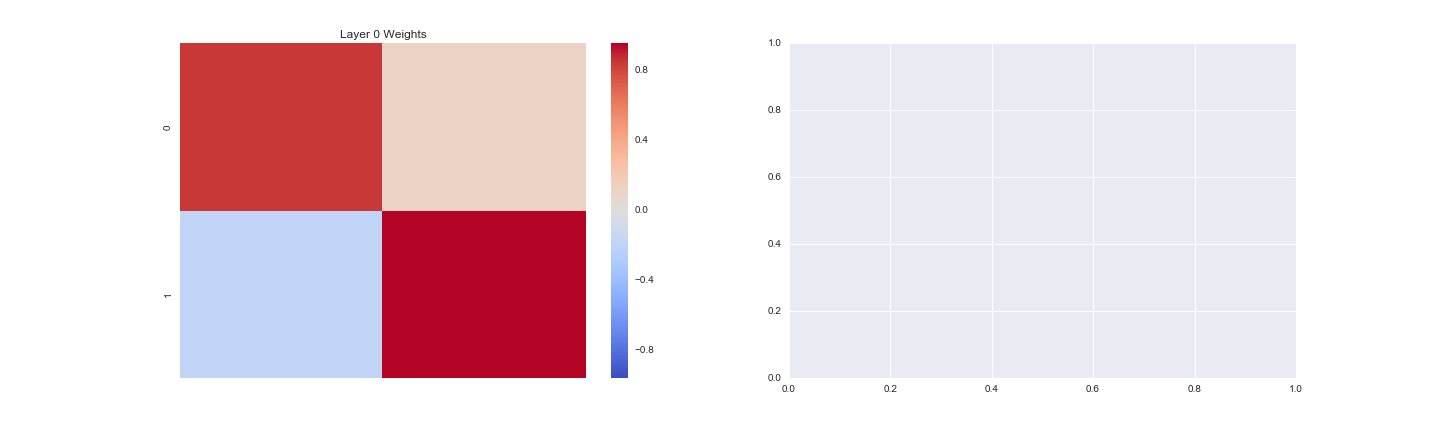
\includegraphics[width=\linewidth]{fig/24-05-2016/clouds/Clouds_GridBendK-closest_Corrector-W.png}
\caption{Correction de Clouds après application d'une transformation linéaire locale}
\label{fig:recap-clouds-GridBend-exhaustive}
\end{figure}

\subexperiment{Alignement appris : cluster plus proche}

{\Large \textbf{Rotation :}} On applique une rotation de 35 degrés par rapport à l'origine $(0,0)$.

\begin{figure}[H] % images
\centering
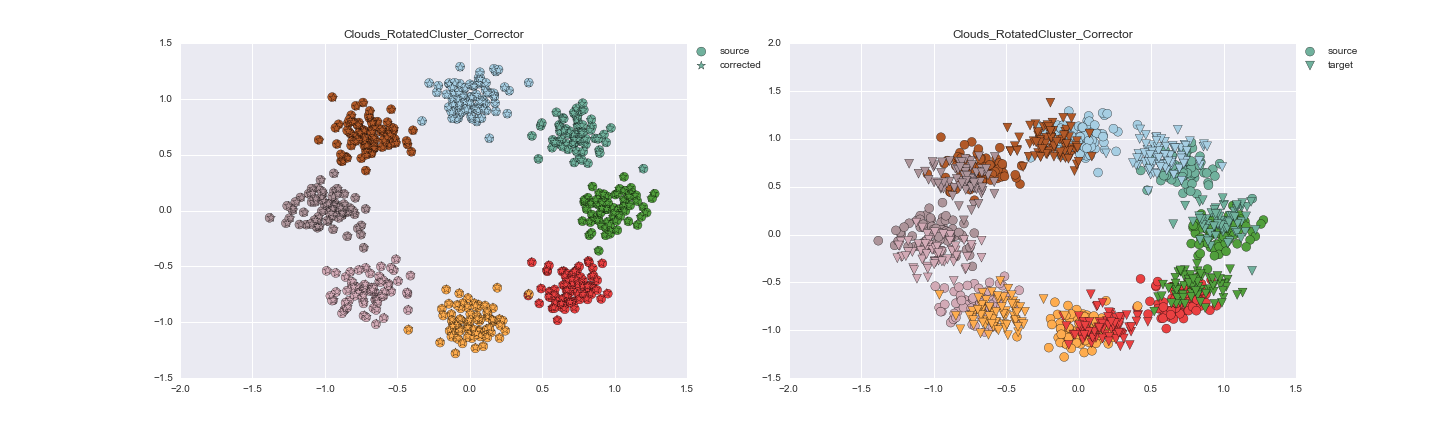
\includegraphics[width=\linewidth]{fig/24-05-2016/clouds/Clouds_RotatedCluster_Corrector-DATA.png}
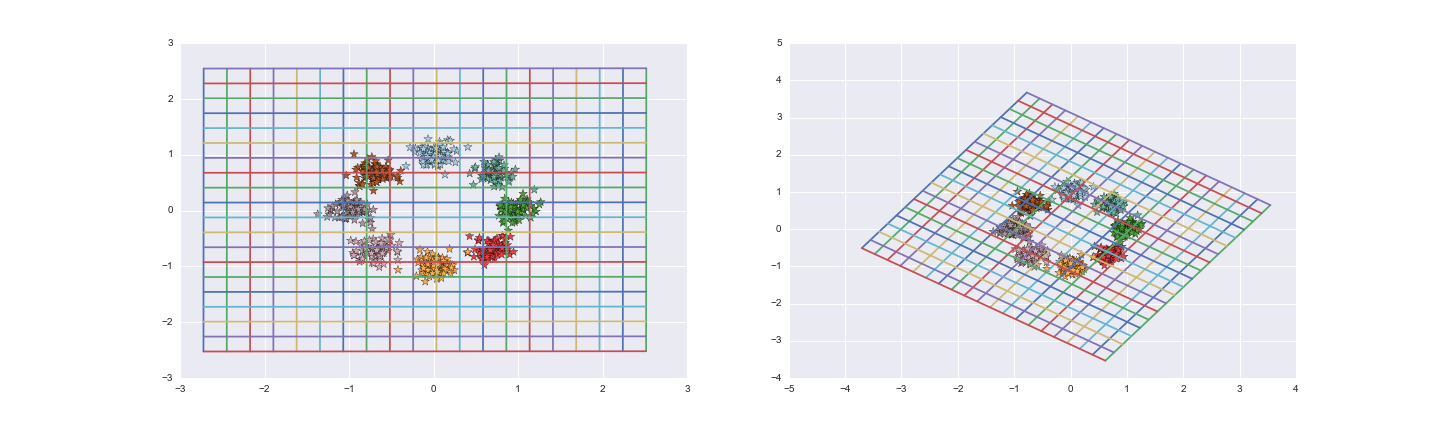
\includegraphics[width=\linewidth]{fig/24-05-2016/clouds/Clouds_RotatedCluster_Corrector-GridCheck.png}
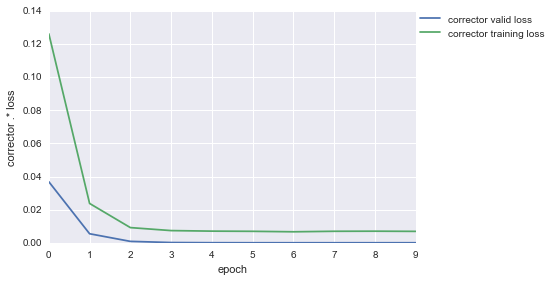
\includegraphics[width=0.45\linewidth]{fig/24-05-2016/clouds/Clouds_RotatedCluster_Corrector-Learning_curve.png}
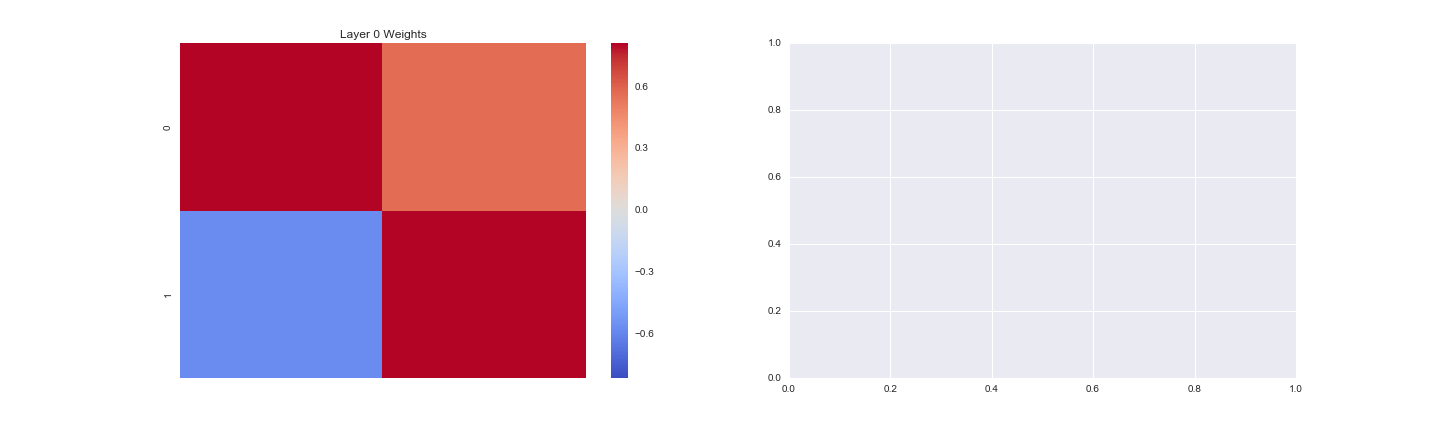
\includegraphics[width=\linewidth]{fig/24-05-2016/clouds/Clouds_RotatedCluster_Corrector-W.png}
\caption{Correction de Clouds après une rotation de 35 degrés par rapport à l'origine avec les plus proches voisins entre les clusters}
\label{fig:recap-clouds-rot-cluster}
\end{figure}

{\Large \textbf{Random matrix :}}

\begin{figure}[H] % images
\centering
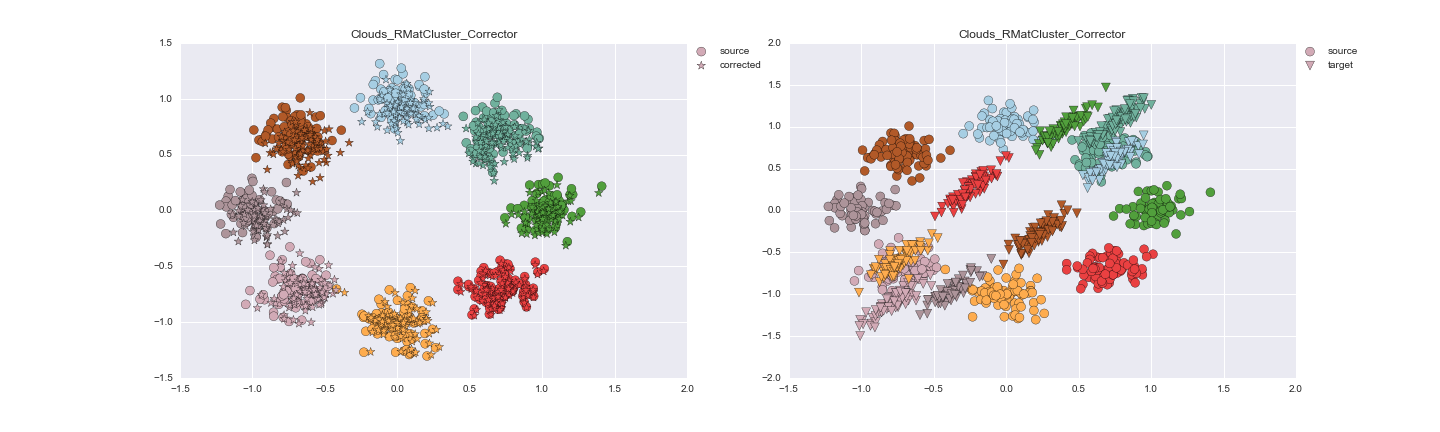
\includegraphics[width=\linewidth]{fig/24-05-2016/clouds/Clouds_RMatCluster_Corrector-DATA.png}
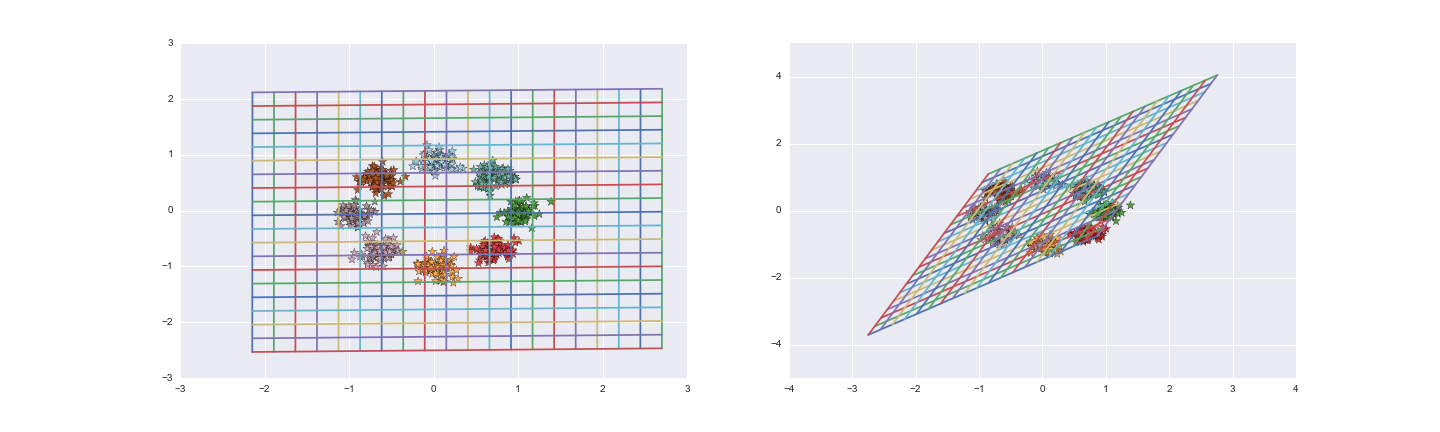
\includegraphics[width=\linewidth]{fig/24-05-2016/clouds/Clouds_RMatCluster_Corrector-GridCheck.png}
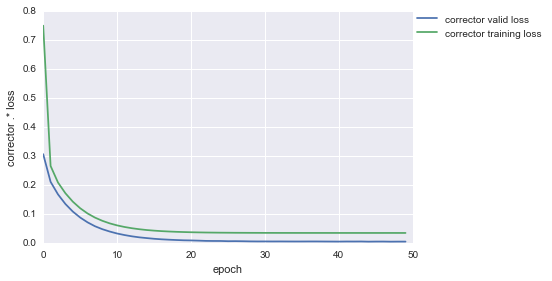
\includegraphics[width=0.45\linewidth]{fig/24-05-2016/clouds/Clouds_RMatCluster_Corrector-Learning_curve.png}
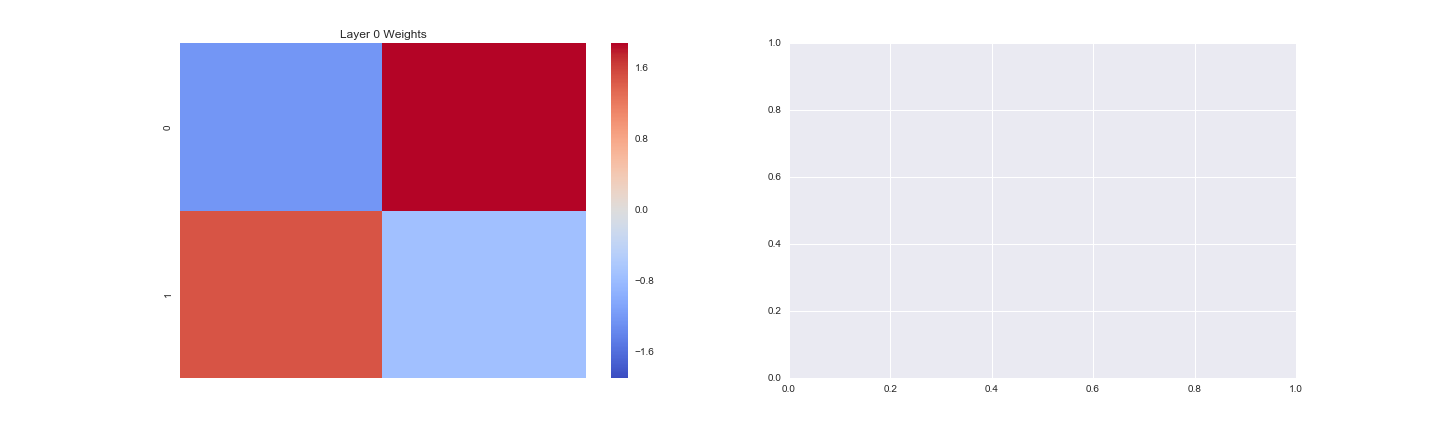
\includegraphics[width=\linewidth]{fig/24-05-2016/clouds/Clouds_RMatCluster_Corrector-W.png}
\caption{Correction de Clouds après multiplication par une matrice générée aléatoirement}
\label{fig:recap-clouds-RMat-cluster}
\end{figure}

{\Large \textbf{Grille tordue :}}

\begin{figure}[H] % images
\centering
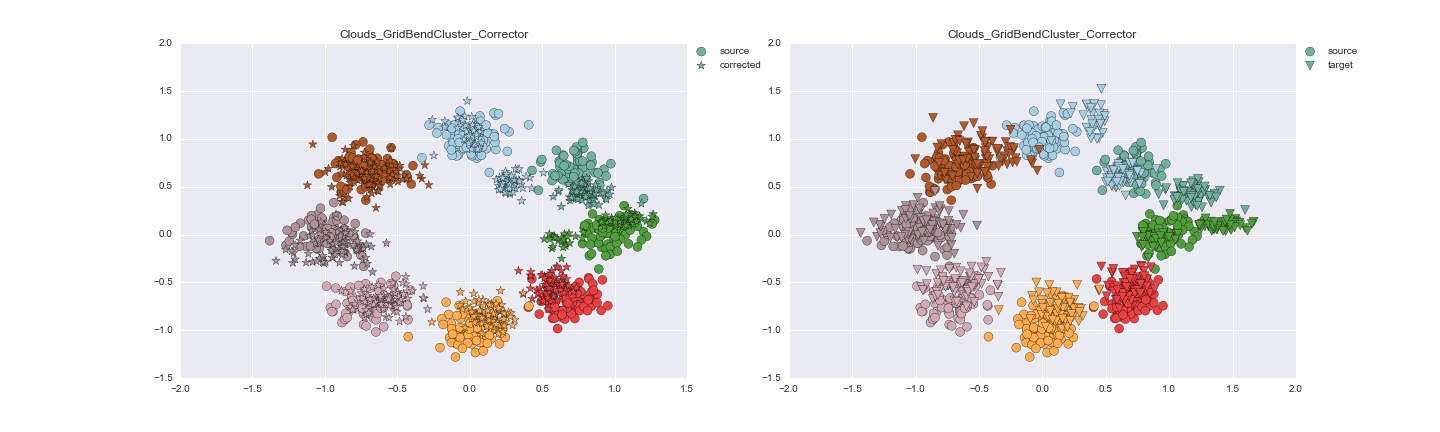
\includegraphics[width=\linewidth]{fig/24-05-2016/clouds/Clouds_GridBendCluster_Corrector-DATA.png}
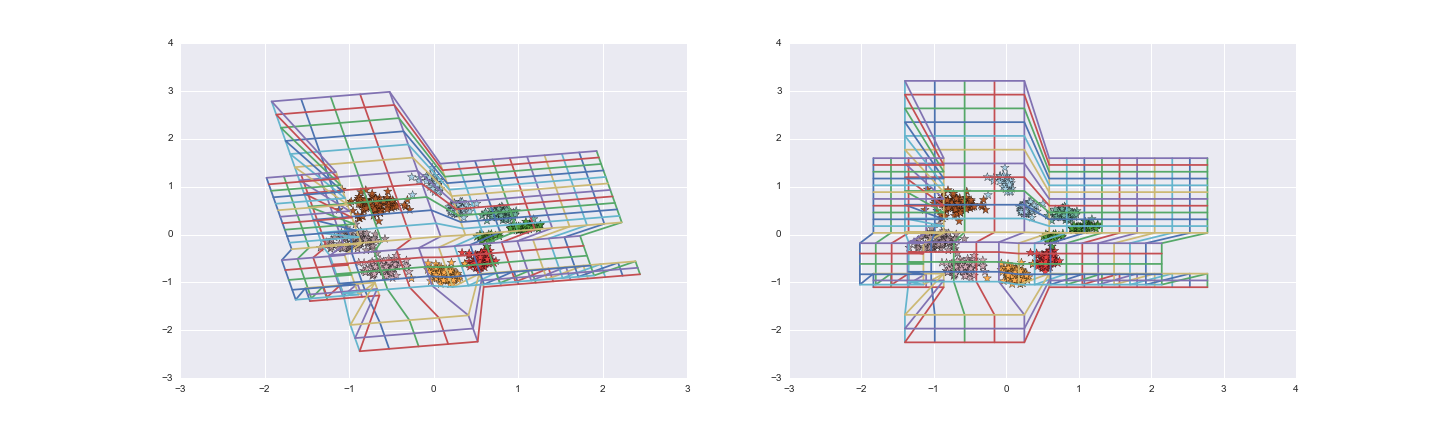
\includegraphics[width=\linewidth]{fig/24-05-2016/clouds/Clouds_GridBendCluster_Corrector-GridCheck.png}
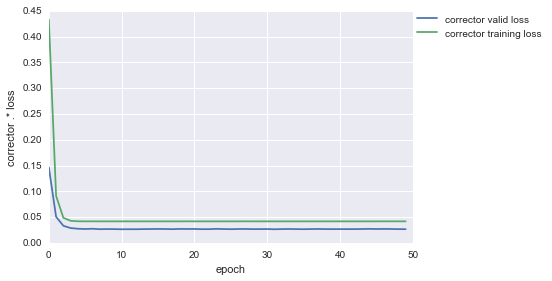
\includegraphics[width=0.45\linewidth]{fig/24-05-2016/clouds/Clouds_GridBendCluster_Corrector-Learning_curve.png}
\includegraphics[width=0.45\linewidth]{fig/24-05-2016/clouds/cloud_grid.png}
\includegraphics[width=\linewidth]{fig/24-05-2016/clouds/Clouds_GridBendCluster_Corrector-W.png}
\caption{Correction de Clouds après application d'une transformation linéaire locale}
\label{fig:recap-clouds-GridBend-cluster}
\end{figure}


%%%%%%%%%%%%%%%%%%%%%%%%%%%%%%%%%%%%%%%%%%%%%%%%%%%%%%%%%%%%%%%%%%%%%%%%%%%%%%
%%%%%% CIRCLES
%%%%%%%%%%%%%%%%%%%%%%%%%%%%%%%%%%%%%%%%%%%%%%%%%%%%%%%%%%%%%%%%%%%%%%%%%%%%%%
\experiment{Circles}

\emph{Circles} est un jouet composé de $n$ classes ...

Toutes ces expériences ont été réaliséeses avec un learning rate de $0.1$ + un moment de $0.9$.


\subexperiment{Alignement connu}

Le cas où l'alignement est connu permet de vérifier que la transformation est facile ou non 
à inverser, les autres méthode ayant peu de chance de faire mieux.

{\Large \textbf{Rotation :}} On applique une rotation de 50 degrés par rapport à l'origine $(0,0)$.

\begin{figure}[H] % images
\centering
\includegraphics[width=\linewidth]{fig/24-05-2016/circles/Circles_RotatedPairwise_Corrector-DATA.png}
\includegraphics[width=\linewidth]{fig/24-05-2016/circles/Circles_RotatedPairwise_Corrector-GridCheck.png}
\includegraphics[width=0.45\linewidth]{fig/24-05-2016/circles/Circles_RotatedPairwise_Corrector-Learning_curve.png}
\includegraphics[width=\linewidth]{fig/24-05-2016/circles/Circles_RotatedPairwise_Corrector-W.png}
\caption{Correction de circles après une rotation de 50 degrés par rapport à l'origine avec alignement connu}
\label{fig:recap-circles-rot-pairwise}
\end{figure}

{\Large \textbf{Random matrix :}}

\begin{figure}[H] % images
\centering
\includegraphics[width=\linewidth]{fig/24-05-2016/circles/Circles_RMatPairwise_Corrector-DATA.png}
\includegraphics[width=\linewidth]{fig/24-05-2016/circles/Circles_RMatPairwise_Corrector-GridCheck.png}
\includegraphics[width=0.45\linewidth]{fig/24-05-2016/circles/Circles_RMatPairwise_Corrector-Learning_curve.png}
\includegraphics[width=\linewidth]{fig/24-05-2016/circles/Circles_RMatPairwise_Corrector-W.png}
\caption{Correction de circles après multiplication par une matrice générée aléatoirement}
\label{fig:recap-circles-RMat-pairwise}
\end{figure}


{\Large \textbf{Grille tordue :}}

\begin{figure}[H] % images
\centering
\includegraphics[width=\linewidth]{fig/24-05-2016/circles/Circles_GridBendPairwise_Corrector-DATA.png}
\includegraphics[width=\linewidth]{fig/24-05-2016/circles/Circles_GridBendPairwise_Corrector-GridCheck.png}
\includegraphics[width=0.45\linewidth]{fig/24-05-2016/circles/Circles_GridBendPairwise_Corrector-Learning_curve.png}
\includegraphics[width=0.45\linewidth]{fig/24-05-2016/circles/circles_grid.png}
\includegraphics[width=\linewidth]{fig/24-05-2016/circles/Circles_GridBendPairwise_Corrector-W.png}
\caption{Correction de circles après application d'une transformation linéaire locale}
\label{fig:recap-circles-GridBend-pairwise}
\end{figure}

\subexperiment{Alignement appris : alignement aléatoire au sein des classes}

{\Large \textbf{Rotation :}} On applique une rotation de 50 degrés par rapport à l'origine $(0,0)$.

\begin{figure}[H] % images
\centering
\includegraphics[width=\linewidth]{fig/24-05-2016/circles/Circles_RotatedClasswise_Corrector-DATA.png}
\includegraphics[width=\linewidth]{fig/24-05-2016/circles/Circles_RotatedClasswise_Corrector-GridCheck.png}
\includegraphics[width=0.45\linewidth]{fig/24-05-2016/circles/Circles_RotatedClasswise_Corrector-Learning_curve.png}
\includegraphics[width=\linewidth]{fig/24-05-2016/circles/Circles_RotatedClasswise_Corrector-W.png}
\caption{Correction de circles après une rotation de 50 degrés par rapport à l'origine avec les plus proches voisins entre les clusters}
\label{fig:recap-circles-rot-classwise}
\end{figure}

{\Large \textbf{Random matrix :}}

\begin{figure}[H] % images
\centering
\includegraphics[width=\linewidth]{fig/24-05-2016/circles/Circles_RMatClasswise_Corrector-DATA.png}
\includegraphics[width=\linewidth]{fig/24-05-2016/circles/Circles_RMatClasswise_Corrector-GridCheck.png}
\includegraphics[width=0.45\linewidth]{fig/24-05-2016/circles/Circles_RMatClasswise_Corrector-Learning_curve.png}
\includegraphics[width=\linewidth]{fig/24-05-2016/circles/Circles_RMatClasswise_Corrector-W.png}
\caption{Correction de circles après multiplication par une matrice générée aléatoirement}
\label{fig:recap-circles-RMat-classwise}
\end{figure}

{\Large \textbf{Grille tordue :}}

\begin{figure}[H] % images
\centering
\includegraphics[width=\linewidth]{fig/24-05-2016/circles/Circles_GridBendClasswise_Corrector-DATA.png}
\includegraphics[width=\linewidth]{fig/24-05-2016/circles/Circles_GridBendClasswise_Corrector-GridCheck.png}
\includegraphics[width=0.45\linewidth]{fig/24-05-2016/circles/Circles_GridBendClasswise_Corrector-Learning_curve.png}
\includegraphics[width=0.45\linewidth]{fig/24-05-2016/circles/circles_grid.png}
\includegraphics[width=\linewidth]{fig/24-05-2016/circles/Circles_GridBendClasswise_Corrector-W.png}
\caption{Correction de circles après application d'une transformation linéaire locale}
\label{fig:recap-circles-GridBend-classwise}
\end{figure}


\subexperiment{Alignement appris : alignement au plus proche voisin au sein des classes}

{\Large \textbf{Rotation :}} On applique une rotation de 50 degrés par rapport à l'origine $(0,0)$.

\begin{figure}[H] % images
\centering
\includegraphics[width=\linewidth]{fig/24-05-2016/circles/Circles_RotatedK-closest_Corrector-DATA.png}
\includegraphics[width=\linewidth]{fig/24-05-2016/circles/Circles_RotatedK-closest_Corrector-GridCheck.png}
\includegraphics[width=0.45\linewidth]{fig/24-05-2016/circles/Circles_RotatedK-closest_Corrector-Learning_curve.png}
\includegraphics[width=\linewidth]{fig/24-05-2016/circles/Circles_RotatedK-closest_Corrector-W.png}
\caption{Correction de circles après une rotation de 50 degrés par rapport à l'origine avec les plus proches voisins entre les clusters}
\label{fig:recap-circles-rot-exhaustive}
\end{figure}

{\Large \textbf{Random matrix :}}

\begin{figure}[H] % images
\centering
\includegraphics[width=\linewidth]{fig/24-05-2016/circles/Circles_RMatK-closest_Corrector-DATA.png}
\includegraphics[width=\linewidth]{fig/24-05-2016/circles/Circles_RMatK-closest_Corrector-GridCheck.png}
\includegraphics[width=0.45\linewidth]{fig/24-05-2016/circles/Circles_RMatK-closest_Corrector-Learning_curve.png}
\includegraphics[width=\linewidth]{fig/24-05-2016/circles/Circles_RMatK-closest_Corrector-W.png}
\caption{Correction de circles après multiplication par une matrice générée aléatoirement}
\label{fig:recap-circles-RMat-exhaustive}
\end{figure}

{\Large \textbf{Grille tordue :}}

\begin{figure}[H] % images
\centering
\includegraphics[width=\linewidth]{fig/24-05-2016/circles/Circles_GridBendK-closest_Corrector-DATA.png}
\includegraphics[width=\linewidth]{fig/24-05-2016/circles/Circles_GridBendK-closest_Corrector-GridCheck.png}
\includegraphics[width=0.45\linewidth]{fig/24-05-2016/circles/Circles_GridBendK-closest_Corrector-Learning_curve.png}
\includegraphics[width=0.45\linewidth]{fig/24-05-2016/circles/circles_grid.png}
\includegraphics[width=\linewidth]{fig/24-05-2016/circles/Circles_GridBendK-closest_Corrector-W.png}
\caption{Correction de circles après application d'une transformation linéaire locale}
\label{fig:recap-circles-GridBend-exhaustive}
\end{figure}

\subexperiment{Alignement appris : cluster plus proche}

{\Large \textbf{Rotation :}} On applique une rotation de 50 degrés par rapport à l'origine $(0,0)$.

\begin{figure}[H] % images
\centering
\includegraphics[width=\linewidth]{fig/24-05-2016/circles/Circles_RotatedCluster_Corrector-DATA.png}
\includegraphics[width=\linewidth]{fig/24-05-2016/circles/Circles_RotatedCluster_Corrector-GridCheck.png}
\includegraphics[width=0.45\linewidth]{fig/24-05-2016/circles/Circles_RotatedCluster_Corrector-Learning_curve.png}
\includegraphics[width=\linewidth]{fig/24-05-2016/circles/Circles_RotatedCluster_Corrector-W.png}
\caption{Correction de circles après une rotation de 50 degrés par rapport à l'origine avec les plus proches voisins entre les clusters}
\label{fig:recap-circles-rot-cluster}
\end{figure}

{\Large \textbf{Random matrix :}}

\begin{figure}[H] % images
\centering
\includegraphics[width=\linewidth]{fig/24-05-2016/circles/Circles_RMatCluster_Corrector-DATA.png}
\includegraphics[width=\linewidth]{fig/24-05-2016/circles/Circles_RMatCluster_Corrector-GridCheck.png}
\includegraphics[width=0.45\linewidth]{fig/24-05-2016/circles/Circles_RMatCluster_Corrector-Learning_curve.png}
\includegraphics[width=\linewidth]{fig/24-05-2016/circles/Circles_RMatCluster_Corrector-W.png}
\caption{Correction de circles après multiplication par une matrice générée aléatoirement}
\label{fig:recap-circles-RMat-cluster}
\end{figure}

{\Large \textbf{Grille tordue :}}

\begin{figure}[H] % images
\centering
\includegraphics[width=\linewidth]{fig/24-05-2016/circles/Circles_GridBendCluster_Corrector-DATA.png}
\includegraphics[width=\linewidth]{fig/24-05-2016/circles/Circles_GridBendCluster_Corrector-GridCheck.png}
\includegraphics[width=0.45\linewidth]{fig/24-05-2016/circles/Circles_GridBendCluster_Corrector-Learning_curve.png}
\includegraphics[width=0.45\linewidth]{fig/24-05-2016/circles/circles_grid.png}
\includegraphics[width=\linewidth]{fig/24-05-2016/circles/Circles_GridBendCluster_Corrector-W.png}
\caption{Correction de circles après application d'une transformation linéaire locale}
\label{fig:recap-circles-GridBend-cluster}
\end{figure}

%%%%%%%%%%%%%%%%%%%%%%%%%%%%%%%%%%%%%%%%%%%%%%%%%%%%%%%%%%%%%%%%%%%%%%%%%%%%%%
%%%%%% X
%%%%%%%%%%%%%%%%%%%%%%%%%%%%%%%%%%%%%%%%%%%%%%%%%%%%%%%%%%%%%%%%%%%%%%%%%%%%%%

\experiment{X}

\emph{X} est un jouet composé de $n$ classes 

Toutes ces expériences ont été réalisées avec un learning rate de $0.1$ + un moment de $0.9$.


\subexperiment{Alignement connu}
Le cas où l'alignement est connu permet de vérifier que la transformation est facile ou non 
à inverser, les autres méthode ayant peu de chance de faire mieux.

{\Large \textbf{Rotation :}} On applique une rotation de 50 degrés par rapport à l'origine $(0,0)$.

\begin{figure}[H] % images
\centering
\includegraphics[width=\linewidth]{fig/24-05-2016/X/X_RotatedPairwise_Corrector-DATA.png}
\includegraphics[width=\linewidth]{fig/24-05-2016/X/X_RotatedPairwise_Corrector-GridCheck.png}
\includegraphics[width=0.45\linewidth]{fig/24-05-2016/X/X_RotatedPairwise_Corrector-Learning_curve.png}
\includegraphics[width=\linewidth]{fig/24-05-2016/X/X_RotatedPairwise_Corrector-W.png}
\caption{Correction de X après une rotation de 50 degrés par rapport à l'origine avec alignement connu}
\label{fig:recap-X-rot-pairwise}
\end{figure}

{\Large \textbf{Random matrix :}}

\begin{figure}[H] % images
\centering
\includegraphics[width=\linewidth]{fig/24-05-2016/X/X_RMatPairwise_Corrector-DATA.png}
\includegraphics[width=\linewidth]{fig/24-05-2016/X/X_RMatPairwise_Corrector-GridCheck.png}
\includegraphics[width=0.45\linewidth]{fig/24-05-2016/X/X_RMatPairwise_Corrector-Learning_curve.png}
\includegraphics[width=\linewidth]{fig/24-05-2016/X/X_RMatPairwise_Corrector-W.png}
\caption{Correction de X après multiplication par une matrice générée aléatoirement}
\label{fig:recap-X-RMat-pairwise}
\end{figure}


{\Large \textbf{Grille tordue :}}

\begin{figure}[H] % images
\centering
\includegraphics[width=\linewidth]{fig/24-05-2016/X/X_GridBendPairwise_Corrector-DATA.png}
\includegraphics[width=\linewidth]{fig/24-05-2016/X/X_GridBendPairwise_Corrector-GridCheck.png}
\includegraphics[width=0.45\linewidth]{fig/24-05-2016/X/X_GridBendPairwise_Corrector-Learning_curve.png}
\includegraphics[width=0.45\linewidth]{fig/24-05-2016/X/X_grid.png}
\includegraphics[width=\linewidth]{fig/24-05-2016/X/X_GridBendPairwise_Corrector-W.png}
\caption{Correction de X après application d'une transformation linéaire locale}
\label{fig:recap-X-GridBend-pairwise}
\end{figure}

\subexperiment{Alignement appris : alignement aléatoire au sein des classes}

{\Large \textbf{Rotation :}} On applique une rotation de 50 degrés par rapport à l'origine $(0,0)$.

\begin{figure}[H] % images
\centering
\includegraphics[width=\linewidth]{fig/24-05-2016/X/X_RotatedClasswise_Corrector-DATA.png}
\includegraphics[width=\linewidth]{fig/24-05-2016/X/X_RotatedClasswise_Corrector-GridCheck.png}
\includegraphics[width=0.45\linewidth]{fig/24-05-2016/X/X_RotatedClasswise_Corrector-Learning_curve.png}
\includegraphics[width=\linewidth]{fig/24-05-2016/X/X_RotatedClasswise_Corrector-W.png}
\caption{Correction de X après une rotation de 50 degrés par rapport à l'origine avec les plus proches voisins entre les clusters}
\label{fig:recap-X-rot-classwise}
\end{figure}

{\Large \textbf{Random matrix :}}

\begin{figure}[H] % images
\centering
\includegraphics[width=\linewidth]{fig/24-05-2016/X/X_RMatClasswise_Corrector-DATA.png}
\includegraphics[width=\linewidth]{fig/24-05-2016/X/X_RMatClasswise_Corrector-GridCheck.png}
\includegraphics[width=0.45\linewidth]{fig/24-05-2016/X/X_RMatClasswise_Corrector-Learning_curve.png}
\includegraphics[width=\linewidth]{fig/24-05-2016/X/X_RMatClasswise_Corrector-W.png}
\caption{Correction de X après multiplication par une matrice générée aléatoirement}
\label{fig:recap-X-RMat-classwise}
\end{figure}

{\Large \textbf{Grille tordue :}}

\begin{figure}[H] % images
\centering
\includegraphics[width=\linewidth]{fig/24-05-2016/X/X_GridBendClasswise_Corrector-DATA.png}
\includegraphics[width=\linewidth]{fig/24-05-2016/X/X_GridBendClasswise_Corrector-GridCheck.png}
\includegraphics[width=0.45\linewidth]{fig/24-05-2016/X/X_GridBendClasswise_Corrector-Learning_curve.png}
\includegraphics[width=0.45\linewidth]{fig/24-05-2016/X/X_grid.png}
\includegraphics[width=\linewidth]{fig/24-05-2016/X/X_GridBendClasswise_Corrector-W.png}
\caption{Correction de X après application d'une transformation linéaire locale}
\label{fig:recap-X-GridBend-classwise}
\end{figure}


\subexperiment{Alignement appris : alignement au plus proche voisin au sein des classes}

{\Large \textbf{Rotation :}} On applique une rotation de 50 degrés par rapport à l'origine $(0,0)$.

\begin{figure}[H] % images
\centering
\includegraphics[width=\linewidth]{fig/24-05-2016/X/X_RotatedK-closest_Corrector-DATA.png}
\includegraphics[width=\linewidth]{fig/24-05-2016/X/X_RotatedK-closest_Corrector-GridCheck.png}
\includegraphics[width=0.45\linewidth]{fig/24-05-2016/X/X_RotatedK-closest_Corrector-Learning_curve.png}
\includegraphics[width=\linewidth]{fig/24-05-2016/X/X_RotatedK-closest_Corrector-W.png}
\caption{Correction de X après une rotation de 50 degrés par rapport à l'origine avec les plus proches voisins entre les clusters}
\label{fig:recap-X-rot-exhaustive}
\end{figure}

{\Large \textbf{Random matrix :}}

\begin{figure}[H] % images
\centering
\includegraphics[width=\linewidth]{fig/24-05-2016/X/X_RMatK-closest_Corrector-DATA.png}
\includegraphics[width=\linewidth]{fig/24-05-2016/X/X_RMatK-closest_Corrector-GridCheck.png}
\includegraphics[width=0.45\linewidth]{fig/24-05-2016/X/X_RMatK-closest_Corrector-Learning_curve.png}
\includegraphics[width=\linewidth]{fig/24-05-2016/X/X_RMatK-closest_Corrector-W.png}
\caption{Correction de X après multiplication par une matrice générée aléatoirement}
\label{fig:recap-X-RMat-exhaustive}
\end{figure}

{\Large \textbf{Grille tordue :}}

\begin{figure}[H] % images
\centering
\includegraphics[width=\linewidth]{fig/24-05-2016/X/X_GridBendK-closest_Corrector-DATA.png}
\includegraphics[width=\linewidth]{fig/24-05-2016/X/X_GridBendK-closest_Corrector-GridCheck.png}
\includegraphics[width=0.45\linewidth]{fig/24-05-2016/X/X_GridBendK-closest_Corrector-Learning_curve.png}
\includegraphics[width=0.45\linewidth]{fig/24-05-2016/X/X_grid.png}
\includegraphics[width=\linewidth]{fig/24-05-2016/X/X_GridBendK-closest_Corrector-W.png}
\caption{Correction de X après application d'une transformation linéaire locale}
\label{fig:recap-X-GridBend-exhaustive}
\end{figure}

\subexperiment{Alignement appris : cluster plus proche}

{\Large \textbf{Rotation :}} On applique une rotation de 50 degrés par rapport à l'origine $(0,0)$.

\begin{figure}[H] % images
\centering
\includegraphics[width=\linewidth]{fig/24-05-2016/X/X_RotatedCluster_Corrector-DATA.png}
\includegraphics[width=\linewidth]{fig/24-05-2016/X/X_RotatedCluster_Corrector-GridCheck.png}
\includegraphics[width=0.45\linewidth]{fig/24-05-2016/X/X_RotatedCluster_Corrector-Learning_curve.png}
\includegraphics[width=\linewidth]{fig/24-05-2016/X/X_RotatedCluster_Corrector-W.png}
\caption{Correction de X après une rotation de 50 degrés par rapport à l'origine avec les plus proches voisins entre les clusters}
\label{fig:recap-X-rot-cluster}
\end{figure}

{\Large \textbf{Random matrix :}}

\begin{figure}[H] % images
\centering
\includegraphics[width=\linewidth]{fig/24-05-2016/X/X_RMatCluster_Corrector-DATA.png}
\includegraphics[width=\linewidth]{fig/24-05-2016/X/X_RMatCluster_Corrector-GridCheck.png}
\includegraphics[width=0.45\linewidth]{fig/24-05-2016/X/X_RMatCluster_Corrector-Learning_curve.png}
\includegraphics[width=\linewidth]{fig/24-05-2016/X/X_RMatCluster_Corrector-W.png}
\caption{Correction de X après multiplication par une matrice générée aléatoirement}
\label{fig:recap-X-RMat-cluster}
\end{figure}

{\Large \textbf{Grille tordue :}}

\begin{figure}[H] % images
\centering
\includegraphics[width=\linewidth]{fig/24-05-2016/X/X_GridBendCluster_Corrector-DATA.png}
\includegraphics[width=\linewidth]{fig/24-05-2016/X/X_GridBendCluster_Corrector-GridCheck.png}
\includegraphics[width=0.45\linewidth]{fig/24-05-2016/X/X_GridBendCluster_Corrector-Learning_curve.png}
\includegraphics[width=0.45\linewidth]{fig/24-05-2016/X/X_grid.png}
\includegraphics[width=\linewidth]{fig/24-05-2016/X/X_GridBendCluster_Corrector-W.png}
\caption{Correction de X après application d'une transformation linéaire locale}
\label{fig:recap-X-GridBend-cluster}
\end{figure}

%%%%%%%%%%%%%%%%%%%%%%%%%%%%%%%%%%%%%%%%%%%%%%%%%%%%%%%%%%%%%%%%%%%%%%%%%%%%%%
%%%%%% MOONS
%%%%%%%%%%%%%%%%%%%%%%%%%%%%%%%%%%%%%%%%%%%%%%%%%%%%%%%%%%%%%%%%%%%%%%%%%%%%%%

\experiment{Moons}

\emph{Moons} est un jouet composé de $n$ classes (nuages de point gaussiens) se partageant 
l'espace sur le cercle unité.

Toutes ces expériences ont été réalisées avec un learning rate de $0.1$ + un moment de $0.9$.


\subexperiment{Alignement connu}
Le cas où l'alignement est connu permet de vérifier que la transformation est facile ou non 
à inverser, les autres méthode ayant peu de chance de faire mieux.

{\Large \textbf{Rotation :}} On applique une rotation de 50 degrés par rapport à l'origine $(0,0)$.

\begin{figure}[H] % images
\centering
\includegraphics[width=\linewidth]{fig/24-05-2016/moons/Moons_RotatedPairwise_Corrector-DATA.png}
\includegraphics[width=\linewidth]{fig/24-05-2016/moons/Moons_RotatedPairwise_Corrector-GridCheck.png}
\includegraphics[width=0.45\linewidth]{fig/24-05-2016/moons/Moons_RotatedPairwise_Corrector-Learning_curve.png}
\includegraphics[width=\linewidth]{fig/24-05-2016/moons/Moons_RotatedPairwise_Corrector-W.png}
\caption{Correction de moons après une rotation de 50 degrés par rapport à l'origine avec alignement connu}
\label{fig:recap-moons-rot-pairwise}
\end{figure}

{\Large \textbf{Random matrix :}}

\begin{figure}[H] % images
\centering
\includegraphics[width=\linewidth]{fig/24-05-2016/moons/Moons_RMatPairwise_Corrector-DATA.png}
\includegraphics[width=\linewidth]{fig/24-05-2016/moons/Moons_RMatPairwise_Corrector-GridCheck.png}
\includegraphics[width=0.45\linewidth]{fig/24-05-2016/moons/Moons_RMatPairwise_Corrector-Learning_curve.png}
\includegraphics[width=\linewidth]{fig/24-05-2016/moons/Moons_RMatPairwise_Corrector-W.png}
\caption{Correction de moons après multiplication par une matrice générée aléatoirement}
\label{fig:recap-moons-RMat-pairwise}
\end{figure}


{\Large \textbf{Grille tordue :}}

\begin{figure}[H] % images
\centering
\includegraphics[width=\linewidth]{fig/24-05-2016/moons/Moons_GridBendPairwise_Corrector-DATA.png}
\includegraphics[width=\linewidth]{fig/24-05-2016/moons/Moons_GridBendPairwise_Corrector-GridCheck.png}
\includegraphics[width=0.45\linewidth]{fig/24-05-2016/moons/Moons_GridBendPairwise_Corrector-Learning_curve.png}
\includegraphics[width=0.45\linewidth]{fig/24-05-2016/moons/moons_grid.png}
\includegraphics[width=\linewidth]{fig/24-05-2016/moons/Moons_GridBendPairwise_Corrector-W.png}
\caption{Correction de moons après application d'une transformation linéaire locale}
\label{fig:recap-moons-GridBend-pairwise}
\end{figure}

\subexperiment{Alignement appris : alignement aléatoire au sein des classes}

{\Large \textbf{Rotation :}} On applique une rotation de 50 degrés par rapport à l'origine $(0,0)$.

\begin{figure}[H] % images
\centering
\includegraphics[width=\linewidth]{fig/24-05-2016/moons/Moons_RotatedClasswise_Corrector-DATA.png}
\includegraphics[width=\linewidth]{fig/24-05-2016/moons/Moons_RotatedClasswise_Corrector-GridCheck.png}
\includegraphics[width=0.45\linewidth]{fig/24-05-2016/moons/Moons_RotatedClasswise_Corrector-Learning_curve.png}
\includegraphics[width=\linewidth]{fig/24-05-2016/moons/Moons_RotatedClasswise_Corrector-W.png}
\caption{Correction de moons après une rotation de 50 degrés par rapport à l'origine avec les plus proches voisins entre les clusters}
\label{fig:recap-moons-rot-classwise}
\end{figure}

{\Large \textbf{Random matrix :}}

\begin{figure}[H] % images
\centering
\includegraphics[width=\linewidth]{fig/24-05-2016/moons/Moons_RMatClasswise_Corrector-DATA.png}
\includegraphics[width=\linewidth]{fig/24-05-2016/moons/Moons_RMatClasswise_Corrector-GridCheck.png}
\includegraphics[width=0.45\linewidth]{fig/24-05-2016/moons/Moons_RMatClasswise_Corrector-Learning_curve.png}
\includegraphics[width=\linewidth]{fig/24-05-2016/moons/Moons_RMatClasswise_Corrector-W.png}
\caption{Correction de moons après multiplication par une matrice générée aléatoirement}
\label{fig:recap-moons-RMat-classwise}
\end{figure}

{\Large \textbf{Grille tordue :}}

\begin{figure}[H] % images
\centering
\includegraphics[width=\linewidth]{fig/24-05-2016/moons/Moons_GridBendClasswise_Corrector-DATA.png}
\includegraphics[width=\linewidth]{fig/24-05-2016/moons/Moons_GridBendClasswise_Corrector-GridCheck.png}
\includegraphics[width=0.45\linewidth]{fig/24-05-2016/moons/Moons_GridBendClasswise_Corrector-Learning_curve.png}
\includegraphics[width=0.45\linewidth]{fig/24-05-2016/moons/moons_grid.png}
\includegraphics[width=\linewidth]{fig/24-05-2016/moons/Moons_GridBendClasswise_Corrector-W.png}
\caption{Correction de moons après application d'une transformation linéaire locale}
\label{fig:recap-moons-GridBend-classwise}
\end{figure}


\subexperiment{Alignement appris : alignement au plus proche voisin au sein des classes}

{\Large \textbf{Rotation :}} On applique une rotation de 50 degrés par rapport à l'origine $(0,0)$.

\begin{figure}[H] % images
\centering
\includegraphics[width=\linewidth]{fig/24-05-2016/moons/Moons_RotatedK-closest_Corrector-DATA.png}
\includegraphics[width=\linewidth]{fig/24-05-2016/moons/Moons_RotatedK-closest_Corrector-GridCheck.png}
\includegraphics[width=0.45\linewidth]{fig/24-05-2016/moons/Moons_RotatedK-closest_Corrector-Learning_curve.png}
\includegraphics[width=\linewidth]{fig/24-05-2016/moons/Moons_RotatedK-closest_Corrector-W.png}
\caption{Correction de moons après une rotation de 50 degrés par rapport à l'origine avec les plus proches voisins entre les clusters}
\label{fig:recap-moons-rot-exhaustive}
\end{figure}

{\Large \textbf{Random matrix :}}

\begin{figure}[H] % images
\centering
\includegraphics[width=\linewidth]{fig/24-05-2016/moons/Moons_RMatK-closest_Corrector-DATA.png}
\includegraphics[width=\linewidth]{fig/24-05-2016/moons/Moons_RMatK-closest_Corrector-GridCheck.png}
\includegraphics[width=0.45\linewidth]{fig/24-05-2016/moons/Moons_RMatK-closest_Corrector-Learning_curve.png}
\includegraphics[width=\linewidth]{fig/24-05-2016/moons/Moons_RMatK-closest_Corrector-W.png}
\caption{Correction de moons après multiplication par une matrice générée aléatoirement}
\label{fig:recap-moons-RMat-exhaustive}
\end{figure}

{\Large \textbf{Grille tordue :}}

\begin{figure}[H] % images
\centering
\includegraphics[width=\linewidth]{fig/24-05-2016/moons/Moons_GridBendK-closest_Corrector-DATA.png}
\includegraphics[width=\linewidth]{fig/24-05-2016/moons/Moons_GridBendK-closest_Corrector-GridCheck.png}
\includegraphics[width=0.45\linewidth]{fig/24-05-2016/moons/Moons_GridBendK-closest_Corrector-Learning_curve.png}
\includegraphics[width=0.45\linewidth]{fig/24-05-2016/moons/moons_grid.png}
\includegraphics[width=\linewidth]{fig/24-05-2016/moons/Moons_GridBendK-closest_Corrector-W.png}
\caption{Correction de moons après application d'une transformation linéaire locale}
\label{fig:recap-moons-GridBend-exhaustive}
\end{figure}

\subexperiment{Alignement appris : cluster plus proche}

{\Large \textbf{Rotation :}} On applique une rotation de 50 degrés par rapport à l'origine $(0,0)$.

\begin{figure}[H] % images
\centering
\includegraphics[width=\linewidth]{fig/24-05-2016/moons/Moons_RotatedCluster_Corrector-DATA.png}
\includegraphics[width=\linewidth]{fig/24-05-2016/moons/Moons_RotatedCluster_Corrector-GridCheck.png}
\includegraphics[width=0.45\linewidth]{fig/24-05-2016/moons/Moons_RotatedCluster_Corrector-Learning_curve.png}
\includegraphics[width=\linewidth]{fig/24-05-2016/moons/Moons_RotatedCluster_Corrector-W.png}
\caption{Correction de moons après une rotation de 50 degrés par rapport à l'origine avec les plus proches voisins entre les clusters}
\label{fig:recap-moons-rot-cluster}
\end{figure}

{\Large \textbf{Random matrix :}}

\begin{figure}[H] % images
\centering
\includegraphics[width=\linewidth]{fig/24-05-2016/moons/Moons_RMatCluster_Corrector-DATA.png}
\includegraphics[width=\linewidth]{fig/24-05-2016/moons/Moons_RMatCluster_Corrector-GridCheck.png}
\includegraphics[width=0.45\linewidth]{fig/24-05-2016/moons/Moons_RMatCluster_Corrector-Learning_curve.png}
\includegraphics[width=\linewidth]{fig/24-05-2016/moons/Moons_RMatCluster_Corrector-W.png}
\caption{Correction de moons après multiplication par une matrice générée aléatoirement}
\label{fig:recap-moons-RMat-cluster}
\end{figure}

{\Large \textbf{Grille tordue :}}

\begin{figure}[H] % images
\centering
\includegraphics[width=\linewidth]{fig/24-05-2016/moons/Moons_GridBendCluster_Corrector-DATA.png}
\includegraphics[width=\linewidth]{fig/24-05-2016/moons/Moons_GridBendCluster_Corrector-GridCheck.png}
\includegraphics[width=0.45\linewidth]{fig/24-05-2016/moons/Moons_GridBendCluster_Corrector-Learning_curve.png}
\includegraphics[width=0.45\linewidth]{fig/24-05-2016/moons/moons_grid.png}
\includegraphics[width=\linewidth]{fig/24-05-2016/moons/Moons_GridBendCluster_Corrector-W.png}
\caption{Correction de moons après application d'une transformation linéaire locale}
\label{fig:recap-moons-GridBend-cluster}
\end{figure}


%----------------------------------------------------------------------------------------
